%% ===========================================================================
%% FAccT 2027 submission.
%% Restructured for the 14-page (excluding references) main-text limit.
%% Endmatter statements sit on the permitted extra page.
%% Appendices are unlimited but reviewers are NOT obligated to read them,
%% so the main text is written to be self-contained.
%%
%% THIS REVISION syncs the paper to the ACN-Data (US) re-run and the bootstrap:
%%   - Tables 2 and 3 carry 95% bootstrap intervals (B=10,000, shared draws).
%%   - The four-site sweep is now five sites; ACN-Data Caltech added.
%%   - Figures oracle_tradeoff / rate_design / scarcity_boundary MUST be the
%%     regenerated versions from experiments/results/figures/, not older copies.
%%   - Tables 2 and 3 use \small and tightened \tabcolsep to fit the intervals
%%     in single-column manuscript format. COMPILE-CHECK BOTH.
%%   - Citation keys synced to the verified .bib file.
%% ===========================================================================

%TC:macro \cite [option:text,text]
%TC:macro \citep [option:text,text]
%TC:macro \citet [option:text,text]
%TC:envir table 0 1
%TC:envir table* 0 1
%TC:envir tabular [ignore] word
%TC:envir displaymath 0 word
%TC:envir math 0 word
%TC:envir comment 0 0

%% FAccT requires anonymised submission. The `anonymous' option is mandatory:
%% submissions that do not comply are rejected without review.
\documentclass[manuscript, screen, review, anonymous]{acmart}

\makeatletter
\def\@parfont{\bfseries}
\makeatother

\usepackage{subcaption}
\usepackage{textcomp}
\captionsetup[subfigure]{font=small,skip=2pt}

\AtBeginDocument{%
  \providecommand\BibTeX{{%
Bib\TeX}}}

\setcopyright{acmlicensed}
\copyrightyear{2027}
\acmYear{2027}
\acmDOI{XXXXXXX.XXXXXXX}
\acmConference[FAccT '27]{ACM Conference on Fairness, Accountability, and Transparency}{June 21--24, 2027}{TBD}
\acmISBN{978-1-4503-XXXX-X/2027/06}

\begin{document}

\title{Revenue-Optimal Rationing Puts Lower-Income EV Drivers Last in Line for Power}

% \title{Subsidizing the Cheapest EV Charging Tariff Relocates the Harm Rather Than Removing It}

%% Anonymised for review. Replace with the real author block at camera-ready.
\author{Anonymous Author(s)}
\affiliation{%
\institution{Anonymous Institution}
\country{}
}
\renewcommand{\shortauthors}{Anonymous}

\begin{abstract}
Public electric vehicle charging is becoming everyday infrastructure just as it reaches the households that cannot charge anywhere else. Renters and residents of multi-unit buildings are roughly half as likely as homeowners to have a garage or driveway where a charger can be installed, so for them the public network is not a convenience but the whole of their access to power. A charging site draws that power through a fixed grid connection, so at busy hours it must ration, and operators already price by tier. We audit what a revenue-optimal allocation does under that scarcity. Rather than test one deployed scheduler, we solve the operator's revenue objective exactly as an offline linear program with full knowledge of the day, so the audit measures a property of the objective itself and not the suboptimality of whichever controller happens to be running. On a simulator calibrated to empirical charging and price data, revenue-optimal rationing systematically underserves the lowest-paying tier. Because tier tracks home-charging access, housing tenure, income, and race, the effect is a disparate impact on already-marginalized drivers, produced by a facially neutral rule rather than by intent.

The finding that matters is about the remedy. A subsidy aimed at the poorest drivers does not remove the harm but relocates it within the tiers it pools. What drives the harm is which tier sits lowest in the price ordering, not how far apart the prices are. Capping the top tier narrows the spread while leaving the budget tier at the bottom, so it barely helps. Only an income-neutral tariff, which dissolves the ordering itself, removes the harm, and its cost falls on the operator's revenue rather than on total energy served. We prove that this is structural. The revenue-optimal allocations are characterized by a nested chain of capacity bounds that depends on the tariff only through the tiers' rank order, which makes both the harm and the failure of the partial remedies theorems about the objective rather than empirical regularities. Every headline quantity carries a bootstrap interval over realized days, and the audit replicates on 27,000 real charging sessions from a US campus network. The harm appears where power binds and not elsewhere, so a regulator can target the remedy at the sites that produce it. We identify the affected drivers, the decision-makers who hold the pricing and capacity levers, and the governance instruments those levers map to, and we release the audit instrument.
\end{abstract}

%% TODO before submission: regenerate the CCS XML block from
%% http://dl.acm.org/ccs.cfm and paste it above these \ccsdesc lines.
\ccsdesc[500]{Social and professional topics~Computing / technology policy}
\ccsdesc[300]{Applied computing~Transportation}
\ccsdesc[100]{Theory of computation~Network flows}

\maketitle

%% ===========================================================================
\section{Introduction}

Charging an Electric Vehicle (EV) away from home is not the same experience for everyone. The drivers who lean hardest on public charging are the ones with no proper charging access at home, which means renters, people in multi-unit buildings, and lower-income households. Availability and price already fall unevenly across income and race~\cite{hsu2021public,khan2022inequitable,caulfield2022measuring}. As electric vehicles move down the income distribution, who public charging serves well turns into a question of equity. It becomes one now rather than later, because the buildout is still under way and the rules governing it are still being written. Federal deployment funding already carries equity conditions on where chargers are sited~\cite{fhwa2023nevi}, and the technical standards that determine how a constrained site splits power among the cars plugged into it are being adopted with priority mechanisms already in them~\cite{ocpp201}. Pricing and rationing at the site level are the part of that settlement no instrument has yet reached.

This paper audits one such rule. A charging site is a scarce-resource allocator. Any one fast charger can ask for more than a hundred kilowatts, and the site's grid connection is usually rated well under what all its chargers could draw at once, so when several cars are plugged in the operator has to ration. That rationing is a shipping product, not a thought experiment. Open Charge Point Protocol (OCPP) smart-charging profiles carry explicit priorities~\cite{ocpp201}, and commercial load-management platforms advertise faster charging for customers on higher subscription or tariff plans when the site connection is constrained~\cite{ampeco2026}. Operators optimize revenue because revenue is measurable and it pays for the site. They already price by tier, through memberships, subscription plans, product tiers, and congestion pricing, and drivers sort into those tiers by budget, with tier membership documented to track income~\cite{drehobl2020high,hsu2021public}. Our question is what a revenue-optimal allocation does to the low-margin tiers once power binds, and we answer it with an exact instrument instead of a heuristic.

The finding is a distributional harm. Under scarcity a revenue-maximizing schedule sends the available power to the higher-margin tiers and lets the lower-margin ones drive off with half-empty batteries. Those tiers skew lower-income, and dependence on public charging is itself concentrated among renters, apartment residents, and drivers of color, so what comes out is a disparate impact on marginalized drivers from a policy that never reads anyone's income. The discrimination is not the operator's, it is the pricing structure's.

\paragraph{Subsidizing the poorest tier moves the harm rather than removing it.}
The first remedy a policymaker reaches for is a subsidy for the poorest drivers, and it fails. It does not close the gap, and once it lifts that tier off the bottom the shortfall simply moves to whichever tier it has been pooled with. The reason is structural and we prove it. What drives the harm is the rank \emph{ordering} of the tiers by price. Whichever tier sits strictly lowest gets starved, so capping the top tier does almost nothing, and the harm goes away only when the ordering does, under an income-neutral tariff. The bill lands on operator revenue and not on total energy delivered, since the grid limit already fixes how much gets served and the objective only settles who receives it.

\paragraph{Contributions.}
Section~\ref{sec:grounding} grounds the harmed group in observable, documented conditions instead of a modeling parameter, tying tiers to home-charging access, housing tenure, and dependence on public charging, with the evidence chain in Appendix~\ref{app:grounding}. Section~\ref{sec:problem} sets the audit up as an exact offline allocation problem and defines measures that tell a systematic between-tier harm apart from day-to-day noise. Section~\ref{sec:findings} proves the structural cause. A chain characterization of the revenue-optimal set (Theorem~\ref{thm:chain}) shows the optimum turns on the tariff only through rank order, which yields the price-ordering mechanism, the failure of the partial fixes, and the scarcity scoping as corollaries, each verified numerically, with proofs in Appendix~\ref{app:proofs}. Every headline number carries a bootstrap interval over realized days. We also replicate the audit on the public Caltech ACN-Data \cite{lee2019acn} release as an independent check against our European demand calibration (Section~\ref{sec:acn}). Section~\ref{sec:practice} places the finding among the decision-makers and governance instruments that can act on it, and we release the audit instrument along with the scripts that test the rank-versus-spread hypothesis and validate the gap estimator. We treat online controllers as a secondary question with two sides, and both answers are affirmative: the fair operating point is reachable, and so is the harmful one, which out-earns the heuristics operators run today (Section~\ref{sec:online-brief}, Appendix~\ref{app:online}).

%% ===========================================================================
\section{Related work}
\label{sec:related}

Three literatures meet here and our contribution sits in the gap between them. We state the positioning compactly and give it in full in Appendix~\ref{app:related}. Empirical work on charging access has established that the \emph{infrastructure} is inequitably placed and priced~\cite{hsu2021public,khan2022inequitable,caulfield2022measuring,yu2025equity,lou2024income}, but not what a site's \emph{allocation rule} does to drivers once they arrive. Sequential and online fair division proposes allocation rules for abstract claimants~\cite{sinclair2023sequential,benade2018make}, and a fair charging-control literature designs them for this physical setting~\cite{ardakanian2013distributed,zeballos2019proportional,danner2021quality}. We audit a deployed rule instead of proposing a new one, and our fairness is across groups, not among individual sessions. From welfare economics we borrow the vocabulary of inequality aversion~\cite{atkinson1970measurement,mo2000fair,moulin2003fair}, and we apply, without extending, the classical theory of flows and polymatroids~\cite{gale1957theorem,edmonds2003submodular,megiddo1974optimal,fujishige2005submodular}. The paper is an audit in the disparate-impact tradition~\cite{feldman2015certifying,barocas2023fairness}, aimed at a physical-resource allocation instead of a classifier. Two things are specific to it. One is the construct-validity chain from an observable price tier to a protected attribute, laid out link by link. The other is the exact offline optimum as instrument, which separates harm caused by the objective from harm caused by one controller's suboptimality.

\section{Background and normative commitments}
\label{sec:background}

We situate the work in energy justice and distributive justice, not in the machinery of fair machine learning, because what is at stake is how a basic service gets distributed across people. The question is which distribution is just, not which algorithm is fastest.

\paragraph{Energy justice.}
Energy justice is usually organized into distributional, procedural, and recognition dimensions~\cite{sovacool2015energy,jenkins2016energy}. Our work is a distributional audit, that asks who gets the scarce good and who does not. It also connects to work on energy burden, where low-income households spend several times the income share on energy that richer households do~\cite{drehobl2020high,bednar2020recognition}. That leaves the procedural and recognition dimensions untouched. We have no participatory input from affected drivers and no account of how they would frame the problem themselves, a limit we return to in Section~\ref{sec:reflexivity} instead of letting the distributional frame stand in for the whole of justice.

\paragraph{Why these fairness definitions, and what each commits to.}
Fairness here is contested, not one number to optimize, so the instrument computes four optimal allocations and lets each encode a different commitment. Revenue-optimal is the status quo under audit, and it encodes the view that willingness to pay should govern access. Utilitarian maximizes total satisfaction, treating a unit of charging as equally valuable whoever receives it. Maximin maximizes the worst-off tier, in the prioritarian spirit of Rawls's difference principle~\cite{rawls2017theory} but not as a faithful implementation of it. Strict equality drives every tier to a common level, and we include it to expose the gap between equalizing and levelling down that a naive maximin hides. Measuring the energy a driver can obtain, rather than the revenue a driver pays, follows the capability approach~\cite{sen2014development}. Appendix~\ref{app:traditions} sets out each tradition, and why we are not neutral about the structure of the choice among them, in full.

\paragraph{Disparate impact, used precisely.}
\label{sec:disparate}
Disparate impact we use in its technical sense: a facially neutral policy, one that does not touch a protected attribute, that still produces a disproportionate adverse effect on a protected group. Our revenue-optimal allocation is neutral in just that way. It optimizes margin-weighted energy and never sees a driver's income, race, or housing status, and the adverse effect on the low-margin tier is what the audit picks up. Whether this counts as a disparate impact on a protected group, or only as a regressive outcome across price tiers, turns on the empirical chain defended in Section~\ref{sec:grounding}, whose links from housing tenure to income to race rest on measured data and whose weakest link is the behavioral one from an operator's price tier to a driver's charging situation. Either reading leaves our structural findings intact, since they concern the tiers' price ordering, which does not change with the label. On the legal register we are equally direct. Retail charging tariffs fall outside the domains where disparate-impact liability is codified, so the term is used in its technical fairness-literature sense~\cite{feldman2015certifying} and not as a claim that any statute covers the conduct. The nearest live instruments are equity conditions attached to publicly funded deployment~\cite{fhwa2023nevi} and the rate-oversight authority of public utility commissions, which is where Section~\ref{sec:practice} sends the remedy.

\paragraph{Rate design.}
Our sharpest lever is the tariff, so we build on the applied economics of electricity pricing, where the distributional incidence of nonlinear and time-varying pricing has been studied directly~\cite{borenstein2012redistributional,burger2020efficiency}. That is the literature in which our recommendation, an income-neutral tariff that strips out the price ordering across tiers, exists as an instrument a regulator actually holds.

%% ===========================================================================
\section{The setting and the harmed group}
\label{sec:grounding}

Whether a disparate-impact audit is credible depends on whether the harmed group is real. We ground it here and give the derivation and evidence chain in Appendix~\ref{app:grounding}.

\paragraph{A simulator calibrated to empirical data.}
We audit on Chargax, which models a station as a tree of power nodes under a hard grid-connection limit~\cite{ponse2025chargax}. Time moves in five-minute steps, an episode is one day of 288 steps, and at each step a controller picks a discrete charging level for every charger and for an on-site battery. Nothing sampled is synthetic. Arrival times, dwell times, per-session energy demand, and the vehicle fleet all come from measured datasets, and the electricity price is the real Netherlands day-ahead series. That calibration is European while the demographic grounding below is American. For the structural claims the mix is fine, since by Theorem~\ref{thm:chain} they hold for any arrival stream and any tariff ordering. The magnitudes are another matter, being a European demand process read through a US affordability structure, so we close the seam by re-running the audit on a second site driven by US data.

\paragraph{An independent US demand calibration.}
\label{sec:acn}
That second site runs on the public Caltech ACN-Data release~\cite{lee2019acn}. We take its arrival process, split between workdays and weekends because a campus has a weekday rhythm that a pooled rate would flatten, together with dwell time and driver-stated energy demand, drawn as a pair from one session so the within-session correlation survives. Where a driver stated a requested energy we use that in preference to delivered energy, since satisfaction is measured against the driver's own target and delivered energy is an \emph{outcome} of a session that may have been power-limited. We keep only the pre-COVID window, because session volume collapses at the March 2020 campus closure. That leaves 27{,}584 sessions across 674 days (Appendix~\ref{app:grounding}). ACN-Data records sessions rather than tariffs or vehicle models, so two inputs stay as they were, the Dutch day-ahead price series and the modeled fleet. The site is an independent US \emph{demand} calibration, then, and not an end-to-end US site.

\paragraph{Tiers as observable conditions, not an abstract multiplier.}
No real operator infers a driver's income and rations on it, and we do not model it that way. What operators run is differentiated pricing, through memberships and subscription tiers, product tiers such as fast versus level two, and dynamic and congestion pricing, each carrying its own per-kilowatt-hour margin. The link from price tier to delivered power is equally deployed. Commercial dynamic-load-management products split a constrained site connection by the customer's subscription or pricing plan~\cite{ampeco2026}, built on the stacked charging-profile priorities in OCPP~\cite{ocpp201}. We read the tier as an observable proxy for a driver's charging situation, and above all for dependence on public and fast charging as against access to cheap charging at home.

\paragraph{Home-charging access is unevenly distributed, and the gradient is documented.}
Even under full electrification, a substantial minority of vehicles are projected to have no reliable home charger~\cite{ge2021there}, and access splits sharply along several axes. By tenure, roughly 81\% of owner-occupied units have a garage or carport against about 39\% of rentals~\cite{doeeere2018}. By dwelling type, about 93\% for single-family homes against 46\% for apartments~\cite{bauer2021charging}. By income, close to 59\% in lower-income communities by 2030 against about 70\% generally~\cite{bauer2021charging}. And by race: majority Black and Hispanic block groups in California have around seven-tenths the odds of any public charger and half the odds of a publicly funded one, controlling for income and housing~\cite{hsu2021public}; disadvantaged communities nationally have far fewer chargers per capita~\cite{yu2025equity}; and Black households rent at roughly twice the white rate~\cite{lou2024income,khan2022inequitable}. Drivers without home charging also pay two to three times as much per kilowatt hour~\cite{borlaug2025economics,eia2025}. The driver stuck in the low-margin, public-reliant tier is therefore disproportionately a renter, an apartment resident, lower-income, and non-white. That is an empirical claim about real charging conditions, not a parameter we chose.

\paragraph{Margins anchored to a documented affordability structure.}
Each tier maps to a household-income tercile from the 2024 American Community Survey~\cite{acs2024}, and its margin is willingness to pay per kilowatt hour relative to the median household under a sub-proportional income elasticity. Residential energy behaves as a necessity, with elasticity strictly between 0 and 1 and a central cluster around 0.3 to 0.6~\cite{schulte2017price,espey2004turning}, and we use 0.6. Out of that come margins of roughly 0.6, 1, and 1.5, a direction the energy-burden gradient corroborates~\cite{drehobl2020high}. Since only the ordering drives the result, as Section~\ref{sec:findings} shows, the elasticity is not load-bearing. Appendix~\ref{app:grounding} carries the full derivation.

\paragraph{Each link in the chain, with its evidence.}
Four links carry the claim, each stated with its evidence in Appendix~\ref{app:grounding}. The chain runs in four steps. First, a driver's price tier reflects how far they depend on public and fast charging, which is an assumption about how drivers sort rather than something we measure. Second, that dependence follows from having no charger at home. Third, home-charging access is sharply stratified by housing tenure, dwelling type, and income. Fourth, tenure and income are themselves stratified by race. The middle links are the strongest, resting on measured access and housing data, and the first is the weakest, being a behavioral assumption about how drivers sort. A correlation carried through several links is weaker than any one of them, so what we claim is the direction and not a one-to-one identity, which is all a disparate-impact reading needs. A reader who finds the first link thin can read regressive allocation for disparate impact throughout. Appendix~\ref{app:grounding} translates the tier gap into an income gap across a range of assumed correlation strengths.

%% ===========================================================================
\section{Problem formulation and audit instrument}
\label{sec:problem}

To keep the difficulty of the problem apart from the difficulty of any one controller, we audit against a clairvoyant offline optimum instead of a heuristic. This section writes that optimum as a linear program, defines the per-driver satisfaction it acts on, gives the objectives encoding the commitments of Section~\ref{sec:background}, states the structural theorem the findings verify, and defines the measures. Proofs sit in Appendix~\ref{app:proofs}.

\paragraph{The allocation problem.}
A day contains a set of charging sessions $\mathcal{I}$, partitioned into tiers $\mathcal{I}=\bigcup_{g\in\mathcal{G}}\mathcal{I}_g$ ordered by per-kilowatt-hour margin, so that $g<g'$ implies $m_g\le m_{g'}$. The audit instantiates $\mathcal{G}=\{1,2,3\}$ as budget, mid, and premium with $m_1<m_2<m_3$, and we keep $\mathcal{G}$ general because Section~\ref{sec:theorem} turns on how tiers group by margin value rather than on how many there are. Time is discretized into steps $t\in\{1,\dots,T\}$ of length $\Delta$ hours ($T=288$, $\Delta=1/12$). Session $i$ belongs to tier $g_i$ and is present over a feasible window $\mathcal{T}_i=\{a_i,\dots,d_i\}$ between arrival and departure. Two further quantities describe the driver and the vehicle rather than the allocation. The desired energy $e_i>0$, in kilowatt hours, is the energy the driver came for, exogenous to the schedule and therefore the target against which satisfaction is measured in~\eqref{eq:sat}. The power cap $\bar p_i>0$, in kilowatts, is the most that session can draw at any step, the lesser of the connector rating and the vehicle's onboard limit, held constant over the session because the program does not model the taper of the charge curve. The site draws through a grid connection of $P$ kilowatts. The decision variable $x_{i,t}\ge 0$ is the power delivered to session $i$ at step $t$, and delivered energy is $E_i=\sum_t \Delta\, x_{i,t}$. The feasible set is
\begin{align}
x_{i,t}&=0 & &\forall i,\ t\notin\mathcal{T}_i, \label{eq:window}\\
0\le x_{i,t}&\le \bar p_i & &\forall i,\ t\in\mathcal{T}_i, \label{eq:cap}\\
\textstyle\sum_t \Delta\, x_{i,t}&\le e_i & &\forall i, \label{eq:demand}\\
\textstyle\sum_i x_{i,t}&\le P & &\forall t. \label{eq:grid}
\end{align}
Constraints~\eqref{eq:window} and~\eqref{eq:cap} are physical, \eqref{eq:demand} says no driver is given more than they asked for, and~\eqref{eq:grid} is the scarcity that forces rationing whenever the power the present sessions could draw at once exceeds $P$.

\paragraph{Per-driver satisfaction.}
For session $i$ we define satisfaction as the fraction of requested energy delivered,
\begin{equation}
u_i=\operatorname{clip}\!\left(\frac{E_i}{e_i},0,1\right),\label{eq:sat}
\end{equation}
which lies in $[0,1]$ and equals $E_i/e_i$ under~\eqref{eq:demand}. We evaluate $u_i$ for every session in the realized stream, not only those who leave satisfied: a driver who reaches the deadline half charged keeps that low score, one still plugged in at the horizon is scored by flushing the station, and one turned away because no charger is free receives a zero. Counting the rejected and the undercharged stops an allocation from looking fair by serving only easy cases. The tier mean is $\bar u_g=|\mathcal{I}_g|^{-1}\sum_{i\in\mathcal{I}_g}u_i$.

\paragraph{Objectives.}
The audit compares the allocations that four commitments produce on the same day. Here $m_{g_i}$ is the per-kilowatt-hour margin of the tier that session $i$ belongs to, a value weight the operator attaches to energy sold into that tier, and $z$ in~\eqref{eq:eq} is an auxiliary variable holding the common satisfaction level that program forces every tier to.
\begin{align}
\text{revenue:}\quad & \textstyle\max_x \sum_i m_{g_i} E_i, \label{eq:rev}\\
\text{utilitarian:}\quad & \textstyle\max_x \sum_i u_i, \label{eq:util}\\
\text{maximin:}\quad & \textstyle\max_{x}\ \min_{g}\ \bar u_g, \label{eq:mm}\\
\text{strict equality:}\quad & \textstyle\max_{x,z}\ z \ \text{ s.t. }\ \bar u_g=z\ \forall g. \label{eq:eq}
\end{align}
Each is a linear program, since $u_i$ and $\bar u_g$ are linear in $x$, and the two distributional programs~\eqref{eq:mm} and~\eqref{eq:eq} act on tier means rather than on individual sessions because the harm under audit is between groups. The revenue program~\eqref{eq:rev} is the deployed status quo we audit, and~\eqref{eq:mm} is solved in the two-stage form given next, never as written.

\paragraph{The maximin must not level down.}
One point of correctness changes the headline. A single program maximizing the worst-off level levels the better-off tiers down to it, reporting a perfectly equal but needlessly impoverished outcome. We therefore solve~\eqref{eq:mm} in two stages: stage one maximizes $z^\star=\max_x\min_g\bar u_g$, and stage two holds it fixed and maximizes total delivered satisfaction subject to $\bar u_g\ge z^\star$. The returned allocation is Pareto efficient, and its worst tier can never fall below what the revenue optimum already delivers. Program~\eqref{eq:eq} is reported only to expose the leveling a naive maximin would produce.

\paragraph{Why the optimum is an upper bound.}
The program relaxes three constraints a causal controller faces: the nonlinear charge curve, round-trip losses, and the discrete assignment of at most $K$ sessions to $K$ connectors. Each relaxation enlarges the feasible set, so the optimum on a day upper-bounds any online policy on that day, the ceiling we audit against. The connector relaxation is why the offline optimum can serve every arriving session a little while an online controller must sometimes reject (Section~\ref{sec:online-brief}).

\paragraph{Uncertainty over realized days.}
\label{sec:bootstrap}
Everything we report is an average over finitely many realized days, so we resample days with replacement, $B=10{,}000$ replicates, and quote $95\%$ percentile intervals. The linear programs are solved once per day, margin vector, and objective, and the bootstrap resamples the cached per-day rows, which attaches each interval to the point estimate it accompanies. Resampling indices are drawn once and shared across every configuration. That keeps quantities paired, and it makes the \emph{difference} between two tariff designs on the same days directly estimable. We use that paired difference, not the overlap of two intervals.

\subsection{The structural theorem}
\label{sec:theorem}

% The findings of Section~\ref{sec:findings} are consequences of a theorem about program~\eqref{eq:rev}, which we state here and prove in Appendix~\ref{app:proofs}. 
For $S\subseteq\mathcal{I}$ let $\hat g(S)$ denote the maximum total energy deliverable to the sessions in $S$ alone under constraints~\eqref{eq:window}--\eqref{eq:grid}, that is, the value of the program maximizing $\sum_{i\in S}E_i$ with $x_{i,t}=0$ for $i\notin S$. Group the tiers by margin value: let $v_1<\dots<v_L$ be the distinct margins, $\mathcal{C}_l$ the union of tiers priced at $v_l$, and $\mathcal{V}_l=\mathcal{C}_l\cup\dots\cup \mathcal{C}_L$ the top sets. Throughout, an \emph{allocation} is any $x$ satisfying \eqref{eq:window}--\eqref{eq:grid}, $E_i=\sum_t\Delta x_{i,t}$ is its delivered energy vector, and $E(S)=\sum_{i\in S}E_i$. Let $A_t=\{i:t\in\mathcal{T}_i\}$ be the sessions present at step $t$, and define
\begin{equation}
f(S)\;=\;\sum_{t}\Delta\,\min\!\Big(P,\ \sum_{i\in S\cap A_t}\bar p_i\Big).
\label{eq:rank}
\end{equation}
The set of feasible delivered-energy vectors is a polymatroid whose rank function is $\hat g$ (Lemma~\ref{lem:polymatroid}, Appendix~\ref{app:proofs}), and linear optimization over a polymatroid is solved by the greedy procedure of Edmonds~\cite{edmonds2003submodular}; specialized to our program this yields Theorem~\ref{thm:chain}.

\begin{lemma}[Exchange]\label{lem:exchange}
At any revenue optimum, for every step $t$ and sessions $i,j\in A_t$ with $m_{g_i}>m_{g_j}$: if $x_{j,t}>0$ then either $x_{i,t}=\bar p_i$ or $E_i=e_i$.
\end{lemma}

\begin{proof}
Otherwise transfer power $\varepsilon>0$ at step $t$ from $j$ to $i$, feasible for small $\varepsilon$ since $x_{i,t}<\bar p_i$ and $E_i<e_i$ and the step total is unchanged, raising the objective by $\Delta(m_{g_i}-m_{g_j})\varepsilon>0$, a contradiction.
\end{proof}

Lemma~\ref{lem:exchange} is the step-level intuition. The theorem is its global form.

\begin{theorem}[Chain characterization]\label{thm:chain}
A feasible allocation is revenue-optimal if and only if it saturates the chain, $E(\mathcal{V}_l)=\hat g(\mathcal{V}_l)$ for every $l$. Consequently every revenue-optimal allocation delivers the same aggregate energy to each margin class, $E(\mathcal{C}_l)=\hat g(\mathcal{V}_l)-\hat g(\mathcal{V}_{l+1})$, and the set of revenue-optimal allocations depends on the tariff only through the partition of tiers into margin classes and their order, never through the margin magnitudes.
\end{theorem}

\begin{theorem}[Totals]\label{thm:base}
Every optimum of any objective that is strictly increasing in each $E_i$, which includes revenue with positive margins, the utilitarian objective~\eqref{eq:util}, and the second stage of the maximin~\eqref{eq:mm}, delivers the same total energy $\hat g(\mathcal{I})$. The strict-equality program~\eqref{eq:eq} is not of this form and can deliver strictly less.
\end{theorem}

\begin{corollary}[Levers]\label{cor:levers}
Under $m_1<m_2<m_3$ the budget tier is the residual claimant, with aggregate exactly $\hat g(\mathcal{I})-\hat g(\mathcal{I}_2\cup\mathcal{I}_3)$ at every revenue optimum. Moreover: (i) capping the premium margin to the middle merges the top classes and leaves that aggregate exactly unchanged; (ii) lifting the budget margin to parity merges the bottom classes, the pooled pair becomes the residual claimant with aggregate $\hat g(\mathcal{I})-\hat g(\mathcal{I}_3)$, and the division within the pool is unconstrained on the optimal face, so the shortfall is relocated within the pool rather than removed; (iii) equal margins collapse the chain to $E(\mathcal{I})=\hat g(\mathcal{I})$, so no tier is a residual claimant and any remaining inequality is selection among optima; (iv) the revenue difference against any fixed alternative allocation is linear in the margins, so the price of fairness moves with the magnitudes while the optimal face does not; (v) if scarcity does not bind, every objective serves every session fully and both the tier gap and the price of fairness are zero.
\end{corollary}

The theorem constrains class \emph{aggregates} and nothing finer, and two things follow from that gap. Tier mean satisfaction can still vary across the optimal face through the within-tier split, which is the solver tie-breaking visible at the third decimal in Table~\ref{tab:grounding}. More consequentially, clause~(ii) of Corollary~\ref{cor:levers} leaves the split within the pooled bottom pair entirely unconstrained, so \emph{which} of the two ends up worst-served after a budget subsidy is a tie-break and not a property of optimality. What the theorem predicts there is the pooled shortfall, not its label, and Section~\ref{sec:mechanism} reports it that way. This also changes what the experiments are for. The elasticity sweep is not a sensitivity analysis that the finding happens to survive but a numerical verification of Theorem~\ref{thm:chain}, and the tariff table verifies Corollary~\ref{cor:levers} clause by clause.

\subsection{Measures}
\label{sec:measures}

Let $\bar u_g^\omega$ be tier $g$'s mean satisfaction on day $\omega$. The \emph{per-day} tier gap is $\gamma_\omega=\max_g\bar u_g^\omega-\min_g\bar u_g^\omega$. The \emph{systematic} (day-averaged) tier gap is
\begin{equation}
\Gamma=\max_g\overline{u}_g-\min_g\overline{u}_g,\qquad
\overline{u}_g=\mathbb{E}_\omega\!\left[\bar u_g^\omega\right].\label{eq:gamma}
\end{equation}
Averaging each tier over days before taking the gap is deliberate: $\Gamma\le\mathbb{E}_\omega[\gamma_\omega]$ with equality only if the same tier is extremal every day, so $\Gamma$ captures a \emph{persistent} between-tier disadvantage and averages away one that rotates. To make that distinction measurable we report the rotation entropy of the worst-off tier. Let $q_g$ be the fraction of days on which $g=\arg\min_{g'}\bar u_{g'}^\omega$; then
\begin{equation}
H=-\frac{1}{\ln|\mathcal{G}|}\sum_{g}q_g\ln q_g\in[0,1].\label{eq:entropy}
\end{equation}
$H\approx 0$ means one tier is always worst, a systematic between-tier harm. $H\approx 1$ means the worst tier rotates evenly, so there is no systematic between-tier harm even if per-day inequality is large. For the deployed-controller and capacity analyses we also report the within-population inequality of the served distribution $\{u_i\}$ via the Gini coefficient, a distinct quantity from $\Gamma$ that measures inequality among individuals rather than between tiers. The revenue price of fairness is $\mathrm{PoF}=(R_{\mathrm{rev}}-R_{\mathrm{maximin}})/R_{\mathrm{rev}}$ with $R=\sum_i m_{g_i} E_i$.

One property of $\Gamma$ matters for reading the tables. It is a max minus a min of \emph{estimated} tier means, so it is biased slightly upward when the tiers are truly equal, and near-zero entries below should be read as equal rather than as a small real inequality.

%% ===========================================================================
\section{Findings}
\label{sec:findings}

The numbers below come from the released run on the scarce reference site, 16 connectors behind a 30-kilowatt grid, over 256 realized days. Under two kilowatts of grid per connector is far below any fast-charging plaza: it is the load-managed regime of many level-two plugs sharing a small feed, precisely the setting commercial load management is sold into~\cite{ampeco2026}, and where the drivers without home charging actually plug in. Corridor sites are sized differently, and their closer analog here is the highway configuration below. The scarcity boundary covers the abundant regimes, and the ACN-Data site of Section~\ref{sec:acn} checks the audit against a demand process we did not calibrate.

\paragraph{The harm is structural, and provably so.}
The elasticity sets how far apart the tier margins sit, and by Theorem~\ref{thm:chain} it cannot touch the harm. By Theorem~\ref{thm:chain} the revenue-optimal set is pinned by the chain $E(\mathcal{V}_l)=\hat g(\mathcal{V}_l)$, which depends on the ordering alone, so per-tier aggregate energy is identical at every margin magnitude and no statistic of the optimal face can drift as the elasticity moves. Behind it is an exchange argument. Whenever the grid limit binds, shifting power from a lower-margin session to an unsatisfied higher-margin one raises revenue, which leaves the lowest-margin tier as residual claimant on every contested step (Lemma~\ref{lem:exchange}). Table~\ref{tab:grounding} and Figure~\ref{fig:grounding} bear this out on the released run. Across the plausible elasticity interval $\Gamma$ stays near $0.545$, moving only in the third decimal, which is precisely the slack the theorem leaves. Per-tier aggregate energies agree across margin magnitudes to machine precision on every audited day, and the lowest-paying tier is worst-served on 91\% of days at every value. Elasticity shifts the price of fairness alone, from about 4\% to 15\%, as Corollary~\ref{cor:levers}(iv) requires, and the harm disappears only at zero spread, as (iii) requires. ACN-Data behaves the same way, the gap sitting between 0.282 and 0.291 for every positive elasticity. So the harm follows from two facts nobody disputes: that a revenue-maximizing operator ranks tiers by margin, and that income sorts drivers into those tiers.

\begin{table}[t]
\centering
\caption{Numerical verification of Theorem~\ref{thm:chain}. $\Gamma$ is flat across the plausible elasticity interval, which changes only the price of fairness, and collapses only at zero spread, where no ordering exists.}
\label{tab:grounding}
\begin{tabular}{lccc}
\toprule
grounding assumption & $\Gamma$ & budget worst & revenue PoF \\
\midrule
elasticity $0.2$ (weak spread)   & 0.546 & 91\% & 4.1\% \\
elasticity $0.6$ (reference)     & 0.545 & 91\% & 10.5\% \\
elasticity $1.0$ (strong spread) & 0.545 & 91\% & 15.0\% \\
elasticity $0$ (no spread)       & 0.012 & 38\% & 0\% \\
\bottomrule
\end{tabular}
\end{table}

The revenue price of fairness is the share of attainable margin-weighted revenue an operator forgoes by moving from the revenue optimum to the corrected maximin,
\begin{equation}
\mathrm{PoF}=\frac{R_{\mathrm{rev}}-R_{\mathrm{maximin}}}{R_{\mathrm{rev}}},\qquad R=\sum_i m_{g_i}E_i,
\label{eq:pof}
\end{equation}
and we abbreviate it PoF in the tables. Two readings of it are worth separating. The denominator is the revenue-optimal value, so PoF measures the cost against the best the objective could do and not against what a given operator currently collects, which is the conservative direction for a regulator sizing a credit. And the comparator is the maximin allocation, so PoF prices \emph{equalization} rather than the flat tariff of Section~\ref{sec:mechanism}, which reaches a similar operating point through the tariff instead of through the scheduler.

\paragraph{The price of fairness is a revenue cost, not a service cost.}
Table~\ref{tab:oracle} and Figure~\ref{fig:oracle} report the optimum. Under revenue-optimal allocation the mid and premium tiers get most of what they ask for while budget sits near forty-one percent, a gap of about 0.55, interval $[0.51, 0.58]$. The corrected maximin brings all three tiers to roughly 0.82 and delivers the \emph{same total energy}. That equality is exact, not approximate, and Theorem~\ref{thm:base} is why: revenue, utilitarian, and corrected maximin are each strictly increasing in delivered energy, so on all 256 days they serve identical totals to solver tolerance and merely redistribute a fixed quantity. Strict equality is the exception the theorem predicts, since forcing equal tier means can block further delivery, and we report it to expose that levelling. Moving to the maximin optimum costs margin-weighted revenue, a median near 10.5\% with an interval of about nine and a half to eleven, while mean satisfaction climbs from about 0.73 to 0.82 and the worst tier from 0.41 to 0.82. That climb is not free. It follows from saturating charging utility, since nobody wants more than a full battery, and the premium tier surrenders about 14 points to pay for it. What is really in tension is operator revenue against the distribution across drivers, not total service against equity. ACN-Data shows the same shape at smaller scale, budget at 0.689 against premium's 0.979, a gap of 0.290 $[0.200, 0.391]$, at a price of fairness of 4.2\% $[2.4, 6.4]$.

\begin{table}[t]
\centering
\small
\setlength{\tabcolsep}{3.5pt}
\caption{The offline audit at the scarce site. Mean satisfaction per tier and value-weighted revenue, each with a $95\%$ bootstrap interval over the 256 days ($B=10{,}000$, indices shared so differences are paired). The revenue optimum starves the budget tier; the corrected maximin equalizes without leveling down and delivers the same energy (Theorem~\ref{thm:base}). Read the maximin and strict-equalization gaps as ``equal''.}
\label{tab:oracle}
\begin{tabular}{lccccc}
\toprule
objective & budget & mid & premium & $\Gamma$ & revenue \\
\midrule
revenue optimal     & 0.41 [0.38, 0.44] & 0.81 [0.79, 0.83] & 0.96 [0.95, 0.96] & 0.55 [0.51, 0.58] & 406 [396, 417] \\
utilitarian         & 0.83 [0.81, 0.85] & 0.83 [0.81, 0.85] & 0.84 [0.82, 0.85] & 0.01 [0.00, 0.04] & 365 [356, 375] \\
tier maximin (true) & 0.82 [0.81, 0.83] & 0.82 [0.81, 0.83] & 0.82 [0.81, 0.83] & 0.00 [0.00, 0.01] & 365 [355, 375] \\
strict equalization & 0.81 [0.80, 0.82] & 0.81 [0.80, 0.82] & 0.81 [0.80, 0.82] & 0.00 [0.00, 0.00] & 359 [349, 369] \\
\bottomrule
\end{tabular}
\end{table}

\begin{figure}[t]
\centering
\begin{subfigure}[b]{0.46\linewidth}
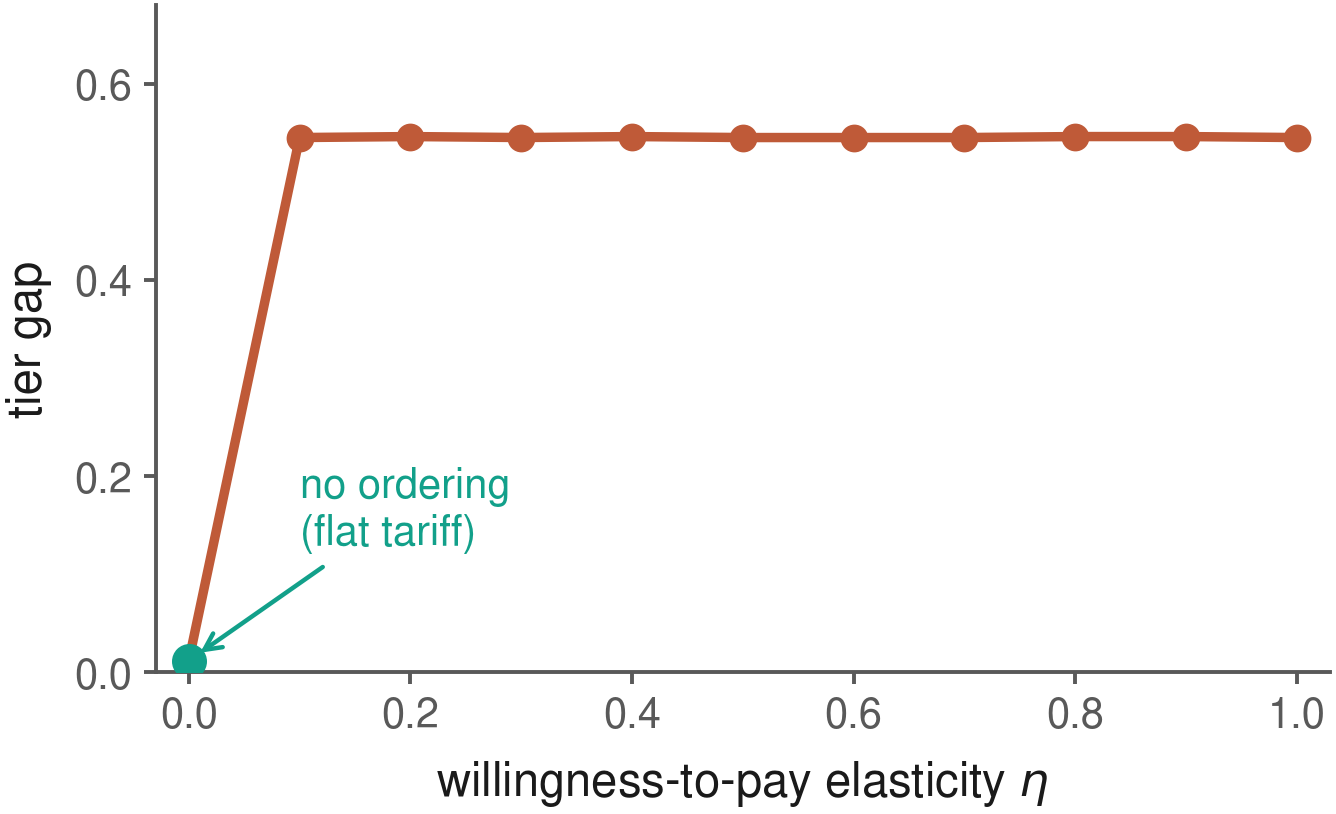
\includegraphics[width=\linewidth]{figures/grounding_invariance.png}
\caption{Ordering, not spread, sets the optimal face.}
\label{fig:grounding}
\end{subfigure}\hfill
\begin{subfigure}[b]{0.46\linewidth}
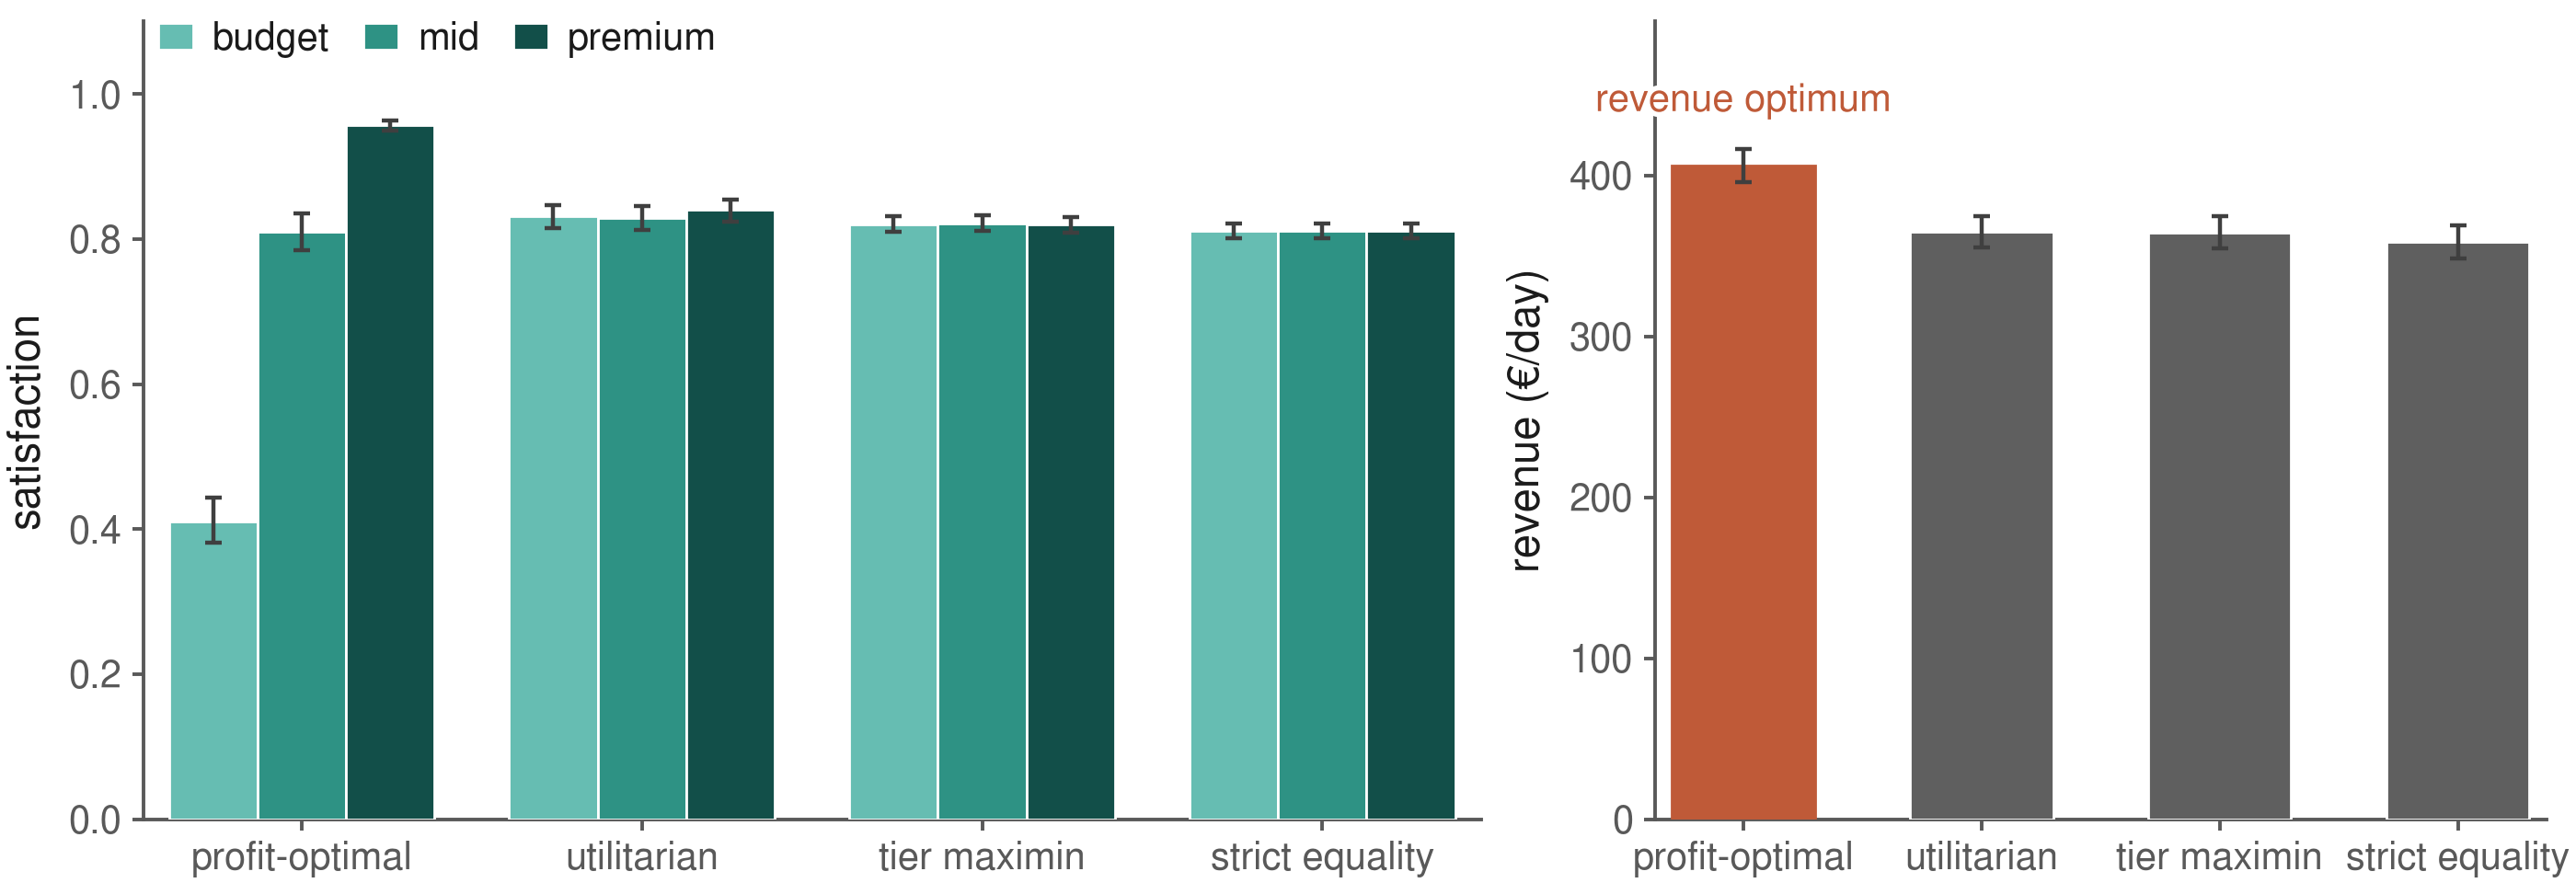
\includegraphics[width=\linewidth]{figures/oracle_tradeoff.png}
\caption{Per-tier service and where the price of fairness is paid.}
\label{fig:oracle}
\end{subfigure}
\caption{The structural claim and the audited objectives. (\subref{fig:grounding}) $\Gamma$ holds near $0.57$ for every $\eta>0$ and collapses only at $\eta=0$, the behavior Theorem~\ref{thm:chain} requires. (\subref{fig:oracle}) Left, per-tier satisfaction, tiers light to dark as budget, mid, premium; right, operator revenue, where the median nine percent cost lands. Whiskers are $95\%$ bootstrap percentile intervals, asymmetric by construction.}
\label{fig:structural}
\end{figure}

\paragraph{The mechanism is rank position, not spread magnitude.}
\label{sec:mechanism}
This is the central finding, and the one that corrects a natural intuition, namely that the harm should scale with how far apart the tier margins are. Table~\ref{tab:tariff} and Figure~\ref{fig:tariff} recompute the revenue-optimal allocation under four tariffs on a fixed day set. Tiers are served in willingness-to-pay order, so budget is starved for as long as it holds the strictly lowest rank, and by how much never enters. The two obvious partial fixes then behave asymmetrically in a way spread magnitude cannot account for. Capping the premium tier at the middle margin squeezes the spread to 0.4 but leaves budget uniquely lowest, so the gap barely shifts, 0.55 to 0.49, and budget stays worst-served across all 10,000 resamples. Corollary~\ref{cor:levers}(i) made visible: budget's aggregate energy is unchanged to machine precision, and what little movement appears in $\Gamma$ comes from the merged upper classes redistributing among themselves. Subsidizing budget to parity squeezes the spread only to 0.5, a \emph{wider} spread, and yet the gap falls to 0.31, because budget is no longer uniquely lowest. The smaller-spread intervention leaves the larger harm.

Both tariffs run on the same realized days, so we can put an interval on the contrast itself instead of on the two gaps separately, which is the stronger test. The paired premium-cap-minus-budget-subsidy difference comes to 0.182, interval $[0.15, 0.20]$, positive in all ten thousand resamples, so the ordering is not an accident of which 256 days we happened to draw. ACN-Data gives 0.141 ($[0.086, 0.203]$), again positive every time. The lever is not the size of the spread. It is whether the budget tier has been rescued from the unique bottom rank.

The subsidy fails differently. It does not leave the harm where it was, it moves the harm inside the pair of tiers it pools, which is Corollary~\ref{cor:levers}(ii) at work. The pooled pair becomes the residual claimant, the division within it is unconstrained on the optimal face, and so which of the two ends up worst is a tie-break. That is what the data show. At the reference site the shortfall lands on the middle tier in a bare majority of resamples, fifty-three percent against budget's forty-seven, which is the coin-flip the corollary predicts rather than a stable relocation, while on ACN-Data the budget tier stays marginally worst, 0.838 against 0.862, close enough to a tie. What generalizes is the pooled shortfall, not its label. A budget-only subsidy leaves most of the harm inside the pool it has created, and only removing the ordering reaches the floor.

Remove the ordering entirely and $\Gamma$ falls to essentially zero, about 0.01 here, the chain collapsing as Corollary~\ref{cor:levers}(iii) says it must. That residual is finite-sample noise and not a floor, as the horizon makes plain: the flat-tariff day-averaged gap falls monotonically from 0.051 at 32 days to 0.044, 0.031, and 0.012 at 64, 128, and 256, while the status-quo gap holds near 0.55 and the flat-tariff worst tier rotates evenly. Flattening leaves one thing behind, the inequality scarcity itself creates, a per-day gap near 0.18 on a rotating tier, which only added capacity reaches. The policy rule is blunt. To remove the harm instead of moving it, remove the ordering. Capping the top tier changes the spread without changing who is at the bottom, and so achieves almost nothing, provably.

\begin{table}[t]
\centering
\small
\setlength{\tabcolsep}{4pt}
\caption{Numerical verification of Corollary~\ref{cor:levers} on one fixed day set. The premium cap compresses the spread \emph{more} than the budget subsidy yet leaves the \emph{larger} gap; the subsidy relocates the shortfall inside the pair it pools; only income-neutral pricing reaches the floor. Brackets are $95\%$ bootstrap intervals; the figure after the worst tier is the share of resamples attributing it there. The decisive contrast is the \emph{paired} difference, $0.182$ $[0.15, 0.20]$, positive in all ten thousand resamples.}
\label{tab:tariff}
\begin{tabular}{lcccc}
\toprule
tariff design & margins & spread & $\Gamma$ & worst tier (share) \\
\midrule
tiered (status quo)      & 0.6, 1.0, 1.5 & 0.9 & 0.55 [0.51, 0.58] & budget (1.00) \\
premium cap to middle    & 0.6, 1.0, 1.0 & 0.4 & 0.49 [0.46, 0.52] & budget (1.00) \\
budget subsidy to parity & 1.0, 1.0, 1.5 & 0.5 & 0.31 [0.29, 0.34] & mid (0.53) \\
income neutral (equal)   & all equal     & 0.0 & 0.01 [0.00, 0.03] & none (roams) \\
\bottomrule
\end{tabular}
\end{table}

\paragraph{The harm is specific to power-scarce sites.}
One site is a thin base for a headline, so we re-run the audit at five stations that vary in charger count, grid size, arrival rate, dwell profile, and fleet, re-running the tariff lever at each. One of them is not a variation of our calibration at all, the ACN-Data campus site of Section~\ref{sec:acn}, driven by real US sessions. The harm turns out not to hold everywhere. The boundary falls between a systematic and a rotating disadvantage, which the rotation entropy $H$ of~\eqref{eq:entropy} makes precise (Table~\ref{tab:sites}, Figure~\ref{fig:scarcity}), and Corollary~\ref{cor:levers}(v) explains why a boundary has to exist at all, since without binding scarcity every objective serves everyone in full. At the three power-bound sites the harm is systematic: budget is worst-served on 91\%, 84\%, and 78\% of days, entropy is low (0.31, 0.49, 0.53), and $\Gamma$ runs about 0.55, 0.29, and 0.21, at a price of fairness near 11\%, 4\%, and 6\%. At a workplace site with long spread dwells and at a low-traffic shopping site, power never binds. There the worst-served tier rotates roughly evenly ($H$ near 0.99 and 0.95) and $\Gamma$ is about 0.005 and 0.04.

No \emph{systematic} between-tier harm shows up at the abundant sites, no tier persistently starved, which is what disparate impact requires. Equal they are not: the shopping site still carries a per-day gap near 0.14, but it falls on a different tier each day, a within-population effect the capacity lever handles and the tariff does not. Across sites the price of fairness tracks the systematic harm, turning positive exactly when rationing by tier pays, and wherever the systematic harm exists the rank mechanism holds, with an income-neutral tariff removing more than 90\% of the gap while a budget-only subsidy leaves most of it. On ACN-Data those figures are 95\% and 51\%, so the mechanism survives a change of demand data and of the sampling scheme behind it, within the scope Section~\ref{sec:acn} sets out. What we can claim, then, is that revenue-optimal allocation \emph{systematically} disadvantages lower-income drivers where power binds and a strict price ordering exists, which lets a regulator target the remedy instead of mandating it everywhere. Put the capacity sweep and the sites on one demand-to-capacity axis (Figure~\ref{fig:severity}) and a sharp within-site boundary appears, together with the fact that a daily ratio cannot see temporal concentration. ACN-Data makes that concrete, its character coming from weekday-morning arrivals no daily total expresses. The dependable flag for a regulator is therefore the price of fairness, computed from the operator's own billing and telemetry.

\begin{table}[t]
\centering
\small
\caption{The scarcity boundary. Low $H$ with large $\Gamma$ marks a systematic between-tier disparate impact (the three power-bound sites); high $H$ with $\Gamma\approx 0$ marks harm that rotates across tiers day to day. The price of fairness is positive exactly at the power-bound sites. ACN-Data is real US session data, not a variation of our calibration. Every row but ACN-Data comes from the 256-day run; the ACN-Data row is the previously released 32-day run, because that configuration needs the Caltech dataset and is skipped when it is absent.}
\label{tab:sites}
\begin{tabular}{lccccc}
\toprule
site & budget worst & $\Gamma$ & per-day gap & $H$ & PoF \\
\midrule
reference (16 ch, 30 kW) & 91\% & 0.545 & 0.59 & 0.31 & 10.5\% \\
ACN-Data (16 ch, 30 kW)  & 84\% & 0.291 & 0.24 & 0.49 & 4.2\% \\
highway (20 ch, 45 kW)   & 78\% & 0.207 & 0.24 & 0.53 & 6.1\% \\
workplace (24 ch, 55 kW) & 39\% & 0.005 & 0.07 & 0.99 & 0\% \\
shopping (8 ch, 16 kW)   & 49\% & 0.040 & 0.14 & 0.95 & 0\% \\
\bottomrule
\end{tabular}
\end{table}

\begin{figure*}[t]
\centering
\begin{subfigure}[b]{0.315\linewidth}
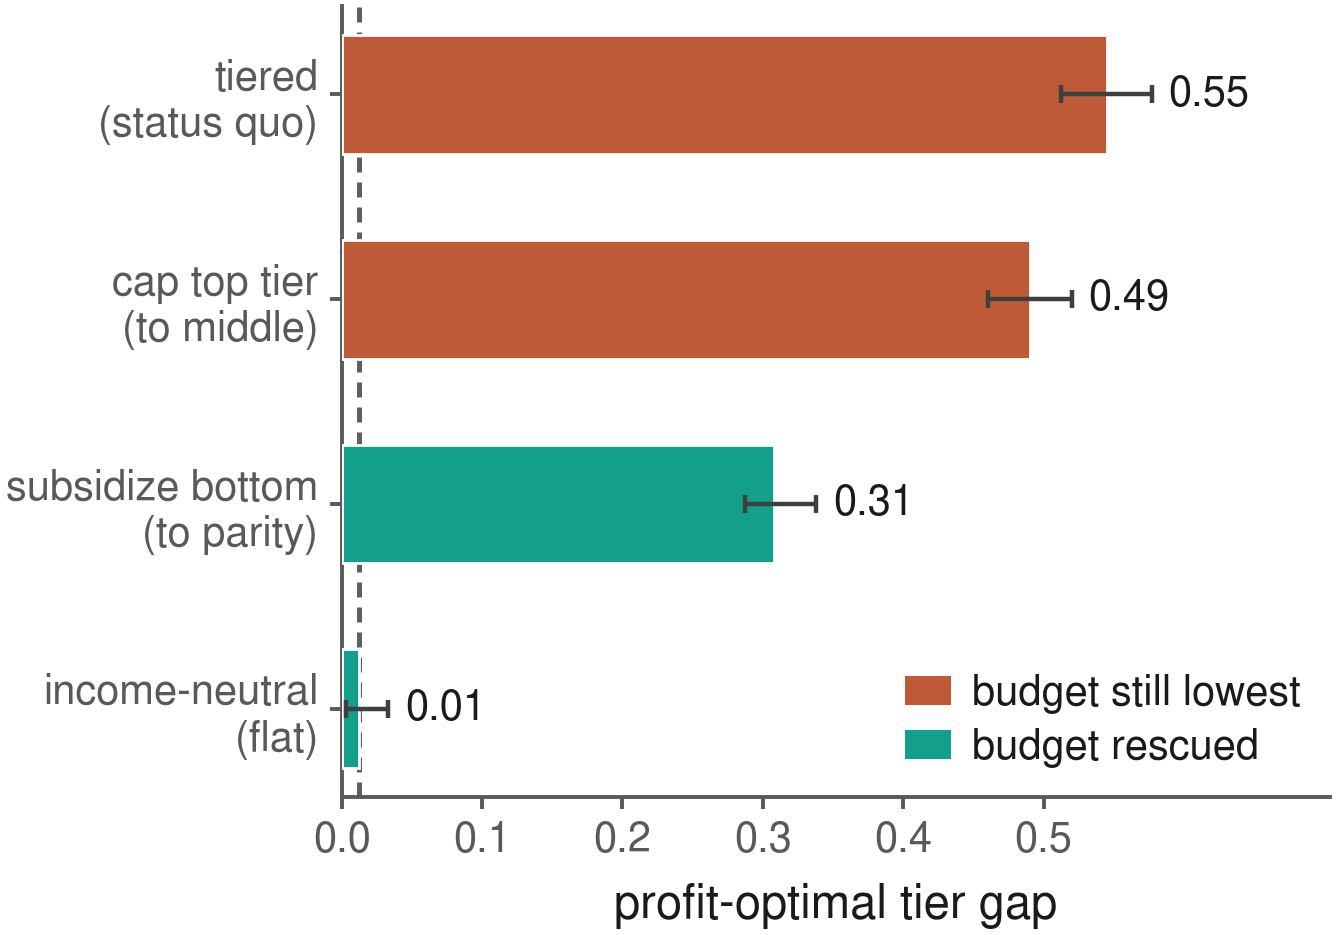
\includegraphics[width=\linewidth]{figures/rate_design.png}
\caption{Rank position, not spread magnitude.}
\label{fig:tariff}
\end{subfigure}\hfill
\begin{subfigure}[b]{0.315\linewidth}
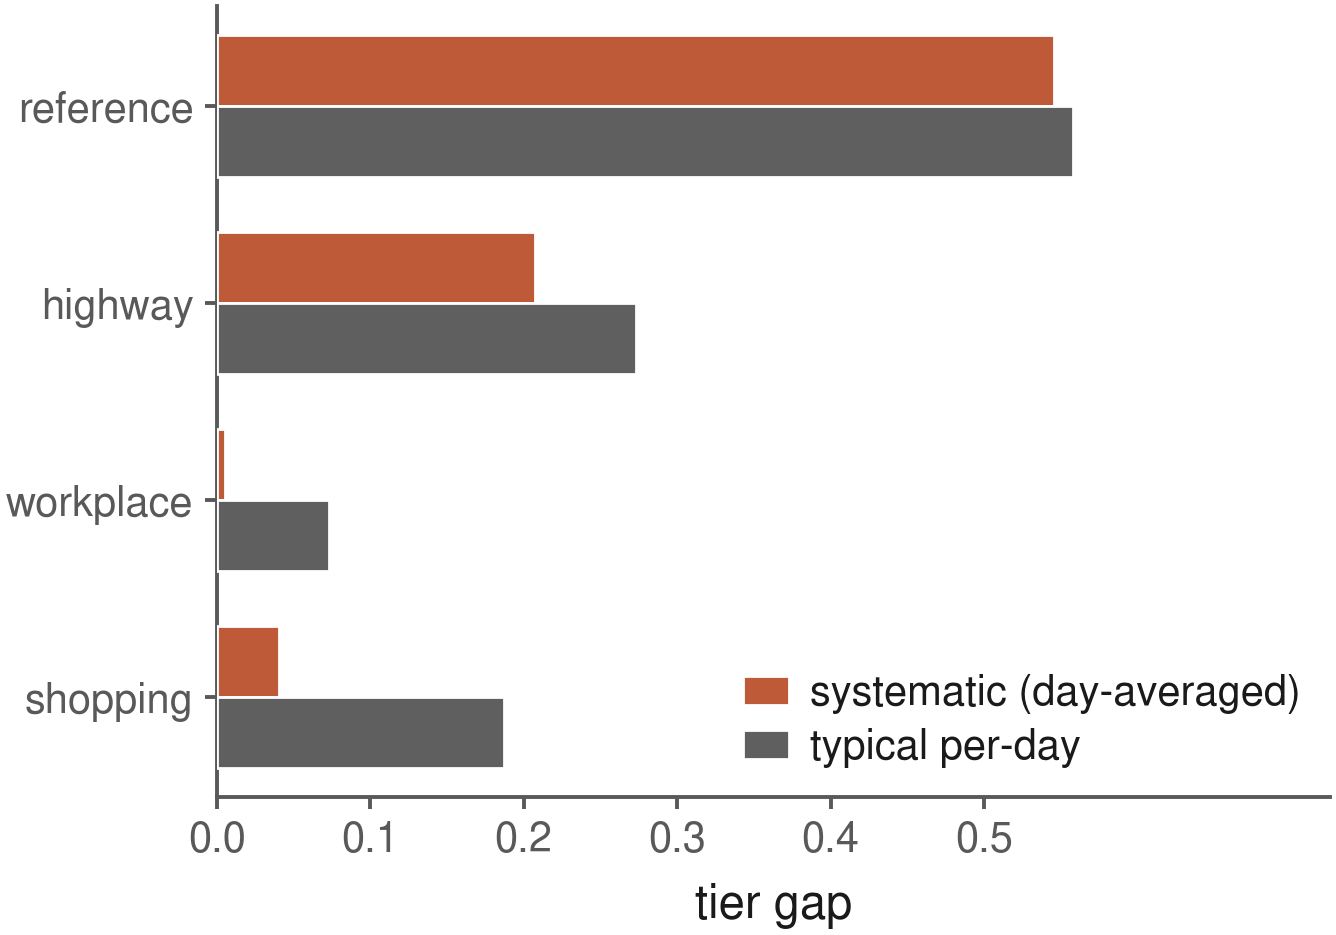
\includegraphics[width=\linewidth]{figures/scarcity_boundary.png}
\caption{Systematic versus rotating disadvantage.}
\label{fig:scarcity}
\end{subfigure}\hfill
\begin{subfigure}[b]{0.315\linewidth}
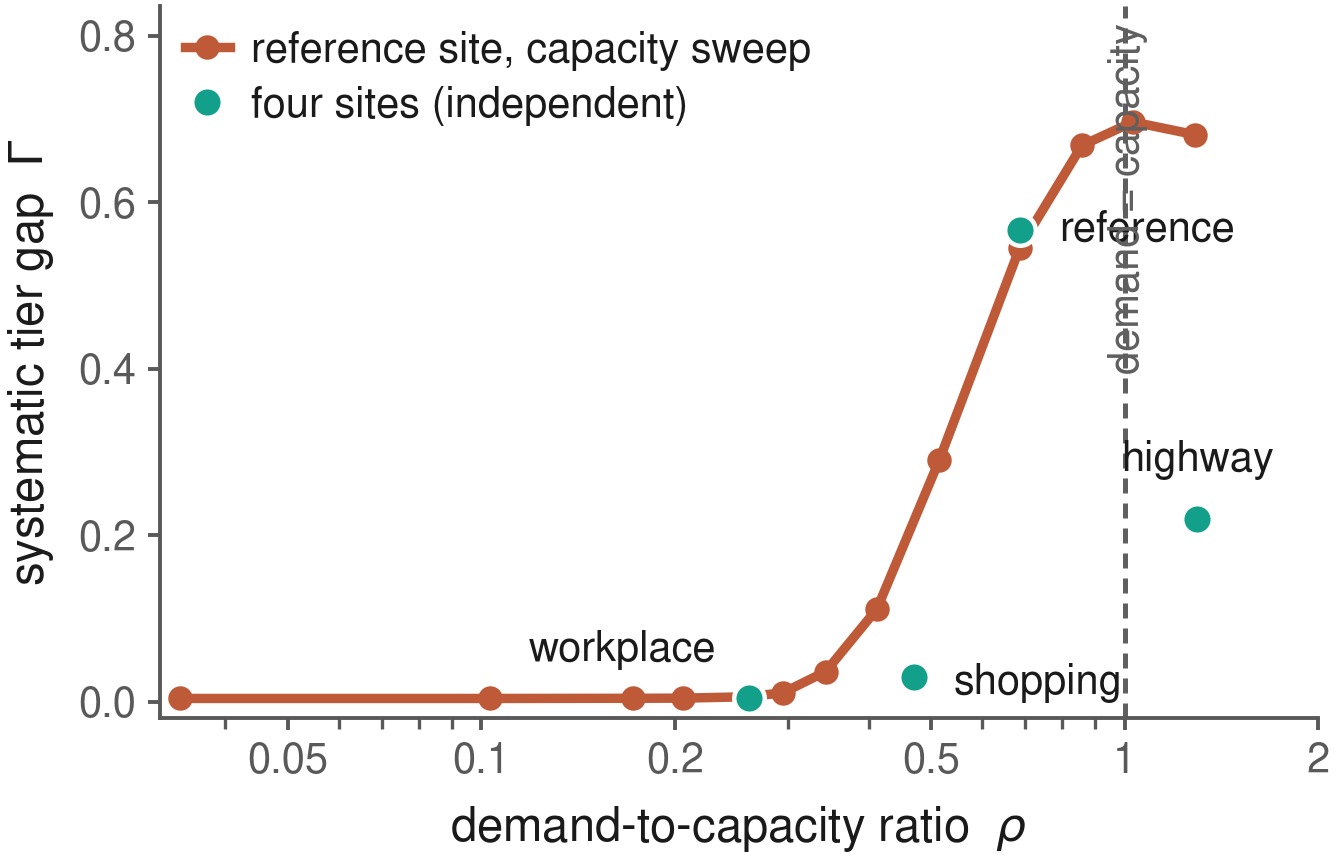
\includegraphics[width=\linewidth]{figures/scarcity_severity.png}
\caption{One severity axis, and its limit.}
\label{fig:severity}
\end{subfigure}
\caption{The mechanism and its scope. (\subref{fig:tariff}) Bars colored by whether the budget tier stays the strictly lowest-priced rank (clay) or is lifted out of it (teal); spreads 0.9, 0.4, 0.5, 0.0, so the premium cap compresses the spread \emph{more} yet leaves the larger gap, and only income-neutral pricing reaches the floor (dashed). (\subref{fig:scarcity}) Systematic $\Gamma$ (clay) against typical per-day gap (gray), power-bound sites first: agreement marks a disparate impact, a large per-day gap with $\Gamma\approx 0$ marks rotating harm. ACN-Data is real US session data. (\subref{fig:severity}) $\Gamma$ against the demand-to-capacity ratio $\rho$: the reference sweep (clay) collapses between $\rho\approx 0.5$ and 0.35, and shopping and highway fall below it because a daily ratio is blind to temporal concentration.}
\label{fig:mechanism}
\end{figure*}

%% --- two levers ------------------------------------------------------------
\paragraph{Grid capacity is a second lever, and it works differently.}
Enough grid capacity dissolves the scarcity that forces rationing in the first place. In the sweep (Figure~\ref{fig:capacity}) the between-tier gap under the optimum reaches essentially zero by about 60 kilowatts, so added power removes the harm this paper audits. The within-population inequality the deployed rule produces also falls, but it flattens at a nonzero Gini floor near 0.30, because a bigger connection removes power rationing without adding chargers, and the residual is drivers turned away when every charger is busy. Since the optimum achieves far lower within-population inequality on the same power, that floor is an online-to-offline and provisioning gap and not a capacity limit, and it is where a better online controller would earn its keep (Section~\ref{sec:online-brief}). ACN-Data reproduces the same thresholds, so they do not depend on the demand process.

These two levers are not orthogonal (Figure~\ref{fig:levers}), and we would rather state the asymmetry than assert a clean split. Raising the connection from 30 to 90 kilowatts cuts \emph{both} the between-tier gap, by about 0.54, and the within-population inequality, by about 0.22, so capacity goes after the root cause. Income-neutral pricing at fixed capacity takes out almost all of the between-tier gap, about 0.53, and barely touches within-population inequality, about 0.06, so pricing is the targeted tool. Where the grid can be sized up, capacity resolves the disparate impact and the power-scarcity share of within-population inequality. Where it cannot, pricing resolves the disparate impact alone. That makes the audit a capacity-planning target as much as a pricing recommendation.

\begin{figure}[t]
\centering
\begin{subfigure}[b]{0.46\linewidth}
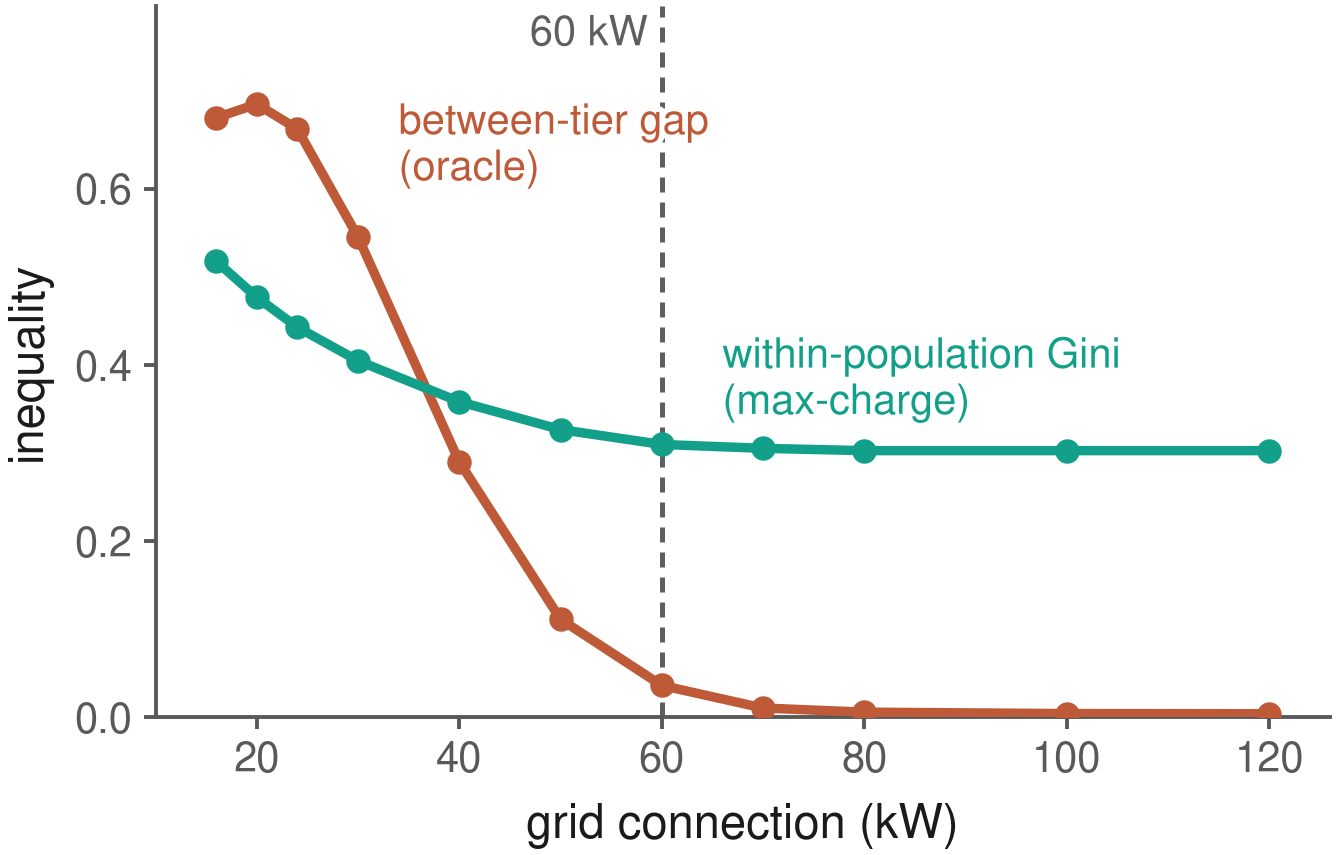
\includegraphics[width=\linewidth]{figures/capacity_threshold.png}
\caption{Capacity and the two inequalities.}
\label{fig:capacity}
\end{subfigure}\hfill
\begin{subfigure}[b]{0.46\linewidth}
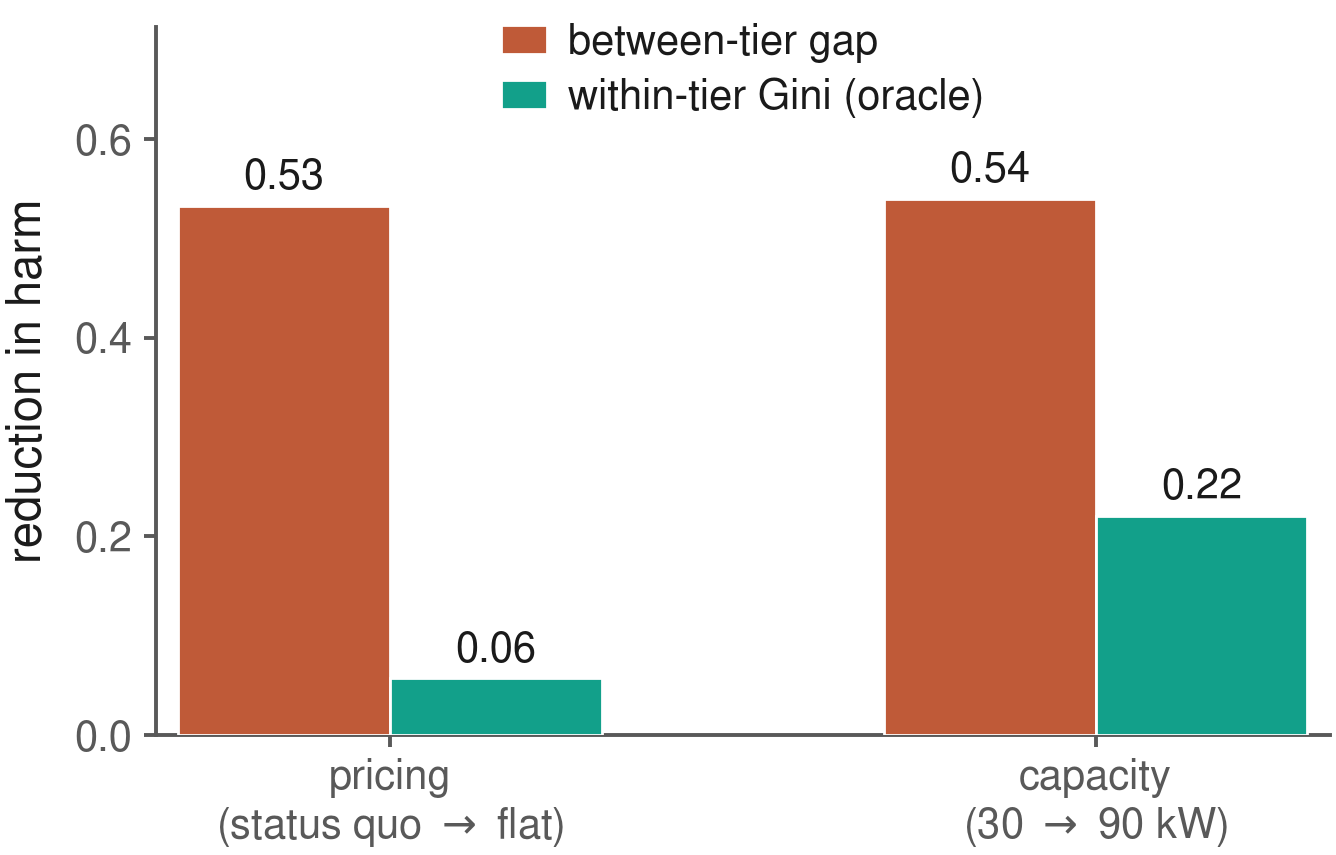
\includegraphics[width=\linewidth]{figures/lever_cross_effects.png}
\caption{The levers are not orthogonal.}
\label{fig:levers}
\end{subfigure}
\caption{The two levers at the reference site. (\subref{fig:capacity}) The between-tier gap under the optimum (clay) reaches essentially zero by about sixty kilowatts (dashed), while the deployed rule's within-population inequality (teal, Gini) flattens near 0.30, a controller and provisioning gap rather than a capacity limit. (\subref{fig:levers}) Pricing removes the between-tier disparate impact but barely touches within-population inequality; capacity reduces both.}
\label{fig:levers-pair}
\end{figure}

%% --- online, in brief ------------------------------------------------------
\subsection{Online realizability}
\label{sec:online-brief}

The offline optimum relaxes constraints a causal controller faces, which invites the reading that the disparate impact is an artifact of clairvoyance. It is not, and showing so requires no learning at all. A margin-greedy heuristic serves connected cars in strict margin order, each tier requesting its feasible maximum and lower tiers receiving whatever the higher tiers leave under the grid limit. This is the myopic online shadow of Theorem~\ref{thm:chain}. It fits in a few lines on any controller that knows a session's price tier, which every billing system does, and it is expressible directly in the stacked charging-profile priorities of the OCPP smart-charging standard that commercial load-management platforms already use for plan-based prioritization~\cite{ocpp201,ampeco2026}.

On the same 256 days it is at once the most profitable heuristic we tried, about 189 euros a day against 181 for max-charge, and the only one that reproduces the harm. The budget tier is worst-served on eighty-four percent of days, with $\Gamma\approx 0.35$ and $H\approx 0.50$, against $\Gamma\le 0.02$ and $H\approx 1.0$ for every non-rationing heuristic, and the online harm is scarcity-scoped exactly as the offline harm is. The incentive to deploy it is therefore live rather than hypothetical, which is the fact Section~\ref{sec:practice} and our ethics statement rest on.

The fair operating point is reachable too, and Appendix~\ref{app:online} gives it in full. A welfare-shaped policy trained with PPO, respecting the connector limit the offline optimum relaxes, beats the strongest rule-based heuristic at the median on profit, inclusive satisfaction, within-population inequality, and rejection rate, dominating on all four at once on seven of ten seeds while rejecting \emph{fewer} drivers. The equity weight is not a between-tier fairness dial, because both the profit and the welfare policies charge broadly instead of rationing hard, so the rationing that produces the offline disparate impact never forms online. 
None of this moves the remedy, which stays with the tariff and the grid connection either way.

%% ===========================================================================
\section{Stakeholders, governance, and the path to practice}
\label{sec:practice}

An audit earns the label socio-technical only by naming who is harmed, who can act, and through what instrument. We do that here.

\paragraph{Who is harmed.}
Those underserved by revenue-optimal rationing are the drivers in the public-reliant low-margin tier, which means disproportionately renters and apartment residents without home charging, lower-income households, and, through the documented correlation between charging access and race, drivers of colour~\cite{hsu2021public,khan2022inequitable}. The harm is concrete. It is a systematically smaller share of the energy they came for, and for a driver with no charger at home that is not an inconvenience but a question of whether the car works tomorrow.

\paragraph{Who holds the levers.}
Three groups hold the pricing lever. Charging network operators set the tariff and run the scheduler. Distribution utilities own the rate designs and low-income programs the charging tariff sits inside. Public utility commissions oversee pricing and can attach equity conditions to procurement and interconnection. The capacity lever belongs to site planners and to the programs funding deployment.

\paragraph{The instruments the levers map to.}
Three real instruments follow. The first is rate regulation. Public charging under scarcity should be priced so that no tier is left strictly lowest, income-neutrally in the limit, and a regulator who cannot mandate a flat tariff can still require the lowest tier to be lifted to parity, which is the same lever in general form. Partial compression that leaves the ordering intact, a top-tier cap for instance, does not work and by Corollary~\ref{cor:levers}(i) cannot. The second is low-income charging tariffs and bill credits, which utilities already run, and which on our reading have to be carried all the way to parity, since a partial credit leaves the shortfall inside the pooled bottom pair. The third is grid-connection sizing in procurement, because sizing above the scarcity range removes the rationing that causes the harm in the first place. Since the harm is specific to power-scarce sites, and a positive price of fairness flags them, the intervention can be targeted, which makes it cheaper to fund and easier to defend. Its bill is a private revenue transfer near ten percent of margin-weighted revenue with no loss of energy served, which bounds any credit a regulator would have to fund and is the number a rate case turns on.

\paragraph{Online controllers change none of this.}
Both directions of online realizability appear in Section~\ref{sec:online-brief}, and the remedy stays with the tariff and the connection either way. The fair allocation needs no exotic control, and the harmful one needs none at all. Today's learned and rule-based controllers steer clear of the harmful operating point only insofar as they fail to ration by margin, and nobody has committed to that.

%% ===========================================================================
\section{Reflexivity and limitations}
\label{sec:reflexivity}

We are the analysts and not the affected community, and the audit shows it. There is no participatory input from the drivers this finding is about, and no account of how renters without home charging would frame the harm or rank the remedies, so what we offer speaks to the distributional dimension of energy justice and stays silent on the procedural and recognition ones. Finding that a group is underserved is not the same as that group being heard.

Modeling ability to pay carries a risk of its own. Segment drivers by willingness to pay and you have built something readable as a price-discrimination tool as easily as an audit of one, since the solver that computes the maximin allocation computes the revenue-optimal one too. We take this up in the ethics statement, and the whole contribution is framed around removing the spread the harmful optimum exploits, but misuse cannot be designed out, and the honest position is that the instrument is dual-use.

ACN-Data narrows the gap between simulation and deployment without closing it. It removes the geographic seam on the demand side, over twenty-seven thousand real US sessions, though not on the price side or the fleet. Our tier-to-income mapping is a model of demand and not a measured demand curve from any operator's customers, and the offline optimum relaxes the nonlinear charge curve, making it a valid upper bound and not a tight one. The bootstrap intervals cover which days were drawn, nothing else. Structural results hold for any arrival stream by Theorem~\ref{thm:chain}, while magnitudes would shift on a given operator's real data, which is why we release the instrument for that re-audit instead of presenting our numbers as final.

%% ===========================================================================
\section{Conclusion}

We audited what revenue-optimal rationing does at a power-scarce charging site and found a disparate impact on the drivers least able to charge at home, produced by a facially neutral pricing structure and not by intent. The remedy is not the obvious one. Subsidizing the poorest drivers relocates the harm inside the tiers it pools, and since the harm tracks the price ordering and not the spread, only removing that ordering removes it, at a cost borne by operator revenue and not by total service. Grid capacity works differently as a second lever, attacking the scarcity itself and cutting both the between-tier harm and the within-population inequality pricing alone leaves behind. The finding is scoped to sites where power binds, and it is structural rather than an artifact of calibration: because the revenue-optimal set turns on the tariff only through the ordering, the harm, the failure of the partial fixes, and the success of the income-neutral tariff are theorems about the objective, verified in simulation rather than discovered there, and replicated on real US session data we did not calibrate.

%% ===========================================================================
%% ENDMATTER. FAccT allows one additional content page for these statements,
%% so they do not count against the 14-page limit.
%% ===========================================================================
\section*{Ethics and adverse impacts statement}

This work audits a distributional harm in a real deployed setting, and the audit instrument is dual-use, which is the primary adverse impact we address. A model of ability-to-pay allocation, of the kind we build to reveal the harm, is structurally the same object an operator would build to optimize price discrimination against low-income drivers, and the revenue-optimal allocation we compute as the thing to be corrected is exactly what an unconstrained profit maximizer would deploy; our appendix shows the harmful operating point is implementable by a trivial online heuristic that out-earns the heuristics operators run today, so the incentive is live, not hypothetical. We have three responses. First, our framing and every recommendation are oriented toward removing the price ordering the harmful optimum exploits, so what a reader is handed is the remedy and the audit that justifies it, not a tuned discrimination engine. Second, we keep tier membership exogenous and never infer a protected attribute at allocation time, and our recommended instruments, income-neutral pricing, low-income tariffs, and capacity sizing, act on pricing structure and infrastructure rather than on any inference of who a driver is, which is both the more effective lever and the one that does not require profiling. Third, we are explicit that the incentive is live, because operators already price by tier, commercial load-management platforms already sell power prioritization by subscription plan under constrained connections~\cite{ampeco2026,ocpp201}, and the margin-greedy controller of Appendix~\ref{app:online} shows the harmful behavior out-earns the heuristics operators run today, so the risk of inaction is not neutral, and an audit that makes the harm measurable and names the remedy is on balance protective even though the instrument could be misused. We also flag a subtler risk, that quantifying ability to pay can reinforce the framing that access to a basic service should track willingness to pay at all, and we take the capability position, in Section~\ref{sec:background}, that access rather than payment is the right space precisely to resist that framing. We use no human-subjects data. The ACN-Data release we build on is public and contains no personal identifiers, and we use only session-level arrival, dwell, and energy fields; the released code contains no personal data.

\section*{Code and data availability}

%% Anonymised mirror for review. The repository is history-scrubbed, so neither the
%% commit metadata nor the remote URL identifies the authors. REPLACE THE PLACEHOLDER
%% BELOW with the URL of the uploaded anonymous mirror before submitting, and replace
%% the whole block with the real repository URL at camera-ready.
The audit instrument, the environment, every script that produces the tables and figures
in this paper, and the released result files are available in an anonymised repository at
\url{https://anonymous.4open.science/r/equicharge-XXXXXX}. The offline audit is CPU-only
and reproduces from a single command. The structural results of
Section~\ref{sec:theorem} are checked numerically day by day rather than asserted, by a
script that verifies the chain characterization and each clause of
Corollary~\ref{cor:levers}, and a second script bounds every reported tier gap over the
revenue-optimal face so no number in this paper depends on which optimal vertex a solver
happens to return. A third script re-derives every numeral printed here from the released
result files, and we ran it as a pre-submission check. The Caltech ACN-Data release is
public and is not redistributed with the repository; the code takes a path to a
locally-fetched copy.

\section*{Generative AI usage statement}

%% REQUIRED by the FAccT Author Guide. VERIFY THIS MATCHES ACTUAL USAGE BEFORE
%% SUBMISSION.
The authors used generative AI tools to assist with the writing of this paper. The authors used AI to edit some phrases to improve coherence and the structure of the paper.

% \clearpage

\bibliographystyle{ACM-Reference-Format}
\bibliography{sample-base}

%% ===========================================================================
%% APPENDICES
%% Unlimited length, placed at the end of the same PDF. Reviewers are not
%% obligated to read them, so nothing here is load-bearing for the main claims.
%% ===========================================================================
\appendix
\section{Related work, in full}
\label{app:related}
Three literatures meet in this paper, and our contribution sits in the gap between them.
\paragraph{Charging access and equity.}
Empirical work documents that public charging is distributed unequally, access correlating with income, housing tenure, and race, and charging deserts concentrating in lower-income and minority neighborhoods~\cite{hsu2021public,khan2022inequitable,caulfield2022measuring,yu2025equity,lou2024income}. That establishes the \emph{infrastructure} is inequitably placed and priced, not what a given site's \emph{allocation rule} does to drivers once they arrive. Our audit holds infrastructure fixed and asks whether the rule rationing scarce power is itself a source of disparate impact.
\paragraph{Fair allocation of scarce resources over time.}
Allocating a limited resource fairly across claimants who arrive over time is classical in operations and mechanism design, studied as sequential and online fair division, where capacity must be committed as demands arrive and fairness trades off against efficiency and against deciding without foreknowledge~\cite{sinclair2023sequential,benade2018make}. That work is method-first: it proposes allocation rules for abstract claimants, without tying them to protected or marginalized real-world groups. We use its normative vocabulary, in particular inequality aversion~\cite{atkinson1970measurement,mo2000fair,moulin2003fair}, and our exact offline optimum is the foreknowledge benchmark such work uses to bound what any causal policy can achieve. Our structural theorem applies rather than extends the classical theory of flows and polymatroids~\cite{gale1957theorem,edmonds2003submodular,megiddo1974optimal,fujishige2005submodular}. Our object differs in two ways: we audit a deployed rule rather than propose a new one, and we ground the affected group empirically, so the audit speaks to a documented protected population.
\paragraph{Fair charging control.}
A separate engineering literature designs fair rationing rules for capacity-limited charging itself: proportionally fair allocation of a constrained feeder~\cite{ardakanian2013distributed}, least-laxity and proportional-fairness policies for garages in overload~\cite{zeballos2019proportional}, and quality-of-service formulations of charging as a service~\cite{danner2021quality}. It shares our physical setting and shows fair online rationing is implementable, supporting the feasibility of our recommendations. It differs in the same two ways as the fair division literature and in a third: its fairness is among individual sessions rather than across groups, and it does not connect the disadvantaged claimants to a documented protected population, which is the step that turns an allocation property into a disparate impact.
\paragraph{Algorithmic disparate impact and audits.}
Disparate impact, a facially neutral rule producing disproportionate harm on a protected group, has a technical formalization with methods to detect and remove it~\cite{feldman2015certifying}, and auditing is now standard for surfacing such harm in deployed systems~\cite{barocas2023fairness}. Ours is an audit in that tradition, applied to a physical-resource allocation rather than a classifier. Two things are specific: the construct-validity chain from an observable price tier to a protected attribute, which we lay out link by link rather than assume, and the use of an exact offline optimum as the instrument, which separates harm produced by the objective from harm produced by a particular controller's suboptimality, so the finding is a property of revenue maximization and not of one scheduler.
\section{Normative traditions, in full}
\label{app:traditions}

Section~\ref{sec:background} names the traditions our four allocation criteria come from. Because our audience spans fields, we state each here, and we are explicit that we use these as allocation criteria in the spirit of the traditions rather than as faithful implementations of them.

Utilitarianism holds that the right allocation maximizes aggregate welfare summed with equal weight across people, which is why our utilitarian objective adds satisfaction and is indifferent to how it is spread. Egalitarianism values equality of outcome as such, the commitment our strict-equality allocation makes literal, and in making it literal it exposes egalitarianism's characteristic failure, that equality can be reached by leveling everyone down. Prioritarianism is the distinct view that a benefit matters more the worse-off its recipient, and Rawls's difference principle is its best-known form, holding that inequalities are acceptable only insofar as they improve the position of the least advantaged~\cite{rawls2017theory}. Our maximin encodes that prioritarian intuition, and we borrow it deliberately rather than claim to apply Rawls's theory. The difference principle is lexical and addresses the primary goods distributed by a society's basic structure, not the rationing of one resource at one charging site, so what we take is the criterion and not the doctrine. The capability approach, due to Sen, locates justice in what a person can actually do or obtain rather than in resources held or utility felt~\cite{sen2014development}, and it is the tradition behind our choice to measure the energy a driver can get rather than the revenue a driver pays.

\paragraph{Why the structure of the choice is not neutral.}
We report all four allocations rather than pick one, because the choice among them is a value choice and different readers will make it differently. We are not, however, neutral about the structure of that choice. Utilitarian efficiency alone is insufficient here, because a utilitarian optimum can leave a minority poorly served whenever doing so raises the total, which is exactly the failure a distributional audit exists to catch, so total satisfaction is a summary we report and not a criterion we endorse. Strict equality is insufficient too, because equalizing by leveling down is equal and worse for all, and our two-stage maximin exists to rule it out. The prioritarian maximin occupies the defensible middle, protecting the worst-off without demanding that the better-off be made worse for the sake of equality alone. Between the mean and the maximin, the Atkinson and alpha-fairness families interpolate along an inequality-aversion parameter, and we use them as a lens on that continuum rather than as a novel method~\cite{atkinson1970measurement,mo2000fair,moulin2003fair}. The capability commitment is not cosmetic, and it is why an allocation that raises revenue while lowering delivered energy to the low-margin tier counts, in our framing, as a harm and not as an efficiency.

\section{Grounding the harmed group, in full}
\label{app:grounding}

\paragraph{Anchoring the margin magnitudes.}
We tie the per-tier margins to a documented affordability structure so the numbers are not chosen for convenience, and we present the derivation in its honest order: real income data first, a real elasticity range second, and the margins as the output. Each tier corresponds to a household-income tercile from the 2024 American Community Survey, whose median household income is about eighty-two thousand dollars, with representative within-tercile incomes near thirty-five, eighty-two, and one hundred sixty-one thousand dollars~\cite{acs2024}. Each tier's margin is its willingness to pay per kilowatt hour relative to the median household, under a sub-proportional income elasticity, because charging is a quasi-necessity and willingness to pay grows more slowly than income. Residential energy is empirically a necessity: its income elasticity lies strictly between zero and one across studies, with a central cluster near zero point three to 0.6~\cite{schulte2017price,espey2004turning}. We use 0.6. The margins are the output of this derivation, approximately 0.6, one, and one point five for the budget, mid, and premium tiers. As Section~\ref{sec:findings} shows, only their ordering, not their magnitudes, drives the result, so the specific value of the elasticity is not load-bearing. The energy-burden gradient corroborates the direction: low-income households below twice the poverty line spend a median of about eight percent of income on home energy against about two percent for higher-income households, a factor of roughly three and a half~\cite{drehobl2020high}. The income terciles, the elasticity, and the energy-burden figures carry real uncertainty. That uncertainty does not reach the finding, because the harm depends on the ordering these numbers produce, not on their magnitudes.

\paragraph{The ACN-Data configuration, in full.}
\label{app:acn}
Section~\ref{sec:acn} summarizes the independent US demand calibration. The underlying release contains 31{,}424 sessions for the Caltech site, of which 27{,}584 fall inside the pre-COVID window we use, 2018-04-25 to 2020-02-29, spanning 674 distinct days, 481 workdays and 193 weekend days. Mean session counts are 48.6 per workday against 21.7 per weekend day, which is why the arrival rate is estimated separately by day type rather than pooled: a single rate would understate weekday contention and overstate weekend contention, and contention is what the audit measures. Median dwell is 313 minutes and median energy demand is 9.94 kilowatt hours. Energy demand is taken from the driver-stated requested field for 12{,}907 sessions and falls back to delivered energy for 14{,}677, and we report that split rather than hide it, because the fallback sessions are the ones where the incumbent controller's rationing could in principle leak into the demand distribution. Dwell and energy are drawn as a pair from the same session. What is \emph{not} taken from ACN-Data is the electricity price, which remains the Netherlands day-ahead series, and the vehicle fleet, which is the modeled US mix, since the release records sessions rather than vehicle models and so does not identify battery capacities or charge curves. The tier segmentation is exogenous on this site exactly as it is on the others.

\paragraph{The tier-to-protected-attribute chain, link by link.}
The claim that the measured tier-level harm is a disparate impact on a protected group rests on a chain of four links. We state each with its evidence and treat the chain as only as strong as its weakest link, rather than assert it whole. Link one: the price tier a driver occupies proxies reliance on public and fast charging, because the low-margin public and level-two products are what a driver without cheap home charging must use. This link is a behavioral assumption about how drivers sort, and it is the one we are least able to measure directly. Link two: reliance on public charging tracks the absence of home charging, and home-charging access splits sharply by housing tenure and dwelling type, roughly eighty-one against thirty-nine percent by owner versus renter and ninety-three against forty-six percent by single-family versus apartment~\cite{doeeere2018,bauer2021charging}. Link three: tenure and dwelling type track income, both directly and through the projected income gradient in charging access itself~\cite{bauer2021charging,drehobl2020high}. Link four: tenure and income track race, with Black households renting at roughly twice the white rate and majority Black and Hispanic areas having markedly lower public-charger access controlling for income and housing~\cite{lou2024income,hsu2021public,yu2025equity}.

The chain is strongest in its middle, links two and three, which rest on measured access and housing data. It is weakest at link one, the mapping from an operator's price tier to a driver's charging situation, which is a behavioral assumption we do not measure in any single operator's data. It is also attenuated overall, because a correlation carried through several links is weaker than any single link. We therefore do not claim a tight one-to-one identity between the budget tier and a protected class. We claim the direction is robust and the association is real and documented, which is what a disparate-impact reading requires, and we retain the weaker regressive-allocation description for a reader who finds link one too thin to carry the protected-attribute label. The structural findings of Section~\ref{sec:findings} do not depend on this chain at all. They concern the price ordering, which produces the tier-level harm whether or not the tier maps cleanly onto income.

\paragraph{Propagation from tier to income, not evidence.}
The gap our audit measures is a disparity across price tiers. To read it as a disparity across income we carry it through the chain above, and we present that step as propagation, not as evidence. Under a symmetric mixing model with correlation strength $\rho$, the income-level gap is exactly $\rho$ times the tier-level gap, so at any assumed correlation the lowest-income bracket is the worst-served and the harm is a fixed fraction of the tier gap: at the reference gap of $0.57$, an income-level gap of $0.45$ at $\rho=0.8$, $0.28$ at $\rho=0.5$, and $0.19$ even at the uninformative $\rho=1/3$. This is arithmetic, and it would be circular to offer it as proof that the correlation is real. The empirical weight for the correlation is the link-by-link chain above, not the mixing model. The model only says how strongly a documented association carries the measured tier-level harm into income space, and the attenuation across links is why we report the translated gap across a range of $\rho$ rather than at a single value.

\section{Proofs}
\label{app:proofs}

\begin{lemma}[The feasible energies form a polymatroid]\label{lem:polymatroid}
A vector $E\ge 0$ with $E_i\le e_i$ for all $i$ is the delivered-energy vector of some allocation if and only if $E(S)\le f(S)$ for every $S\subseteq\mathcal{I}$. Consequently the set $\mathcal{P}$ of feasible delivered-energy vectors is the intersection of the polymatroid of $f$ with the box $\{E\le e\}$, which is itself a polymatroid, and $\hat g(S)=\max\{E(S):E\in\mathcal{P},\ E_j=0\ \forall j\notin S\}$ is its rank function.
\end{lemma}

\begin{proof}[Proof of Lemma~\ref{lem:polymatroid}]
Realizing $E$ is a transportation problem on the bipartite network from sessions to steps, with arc $(i,t)$ of capacity $\Delta\bar p_i$ present iff $t\in\mathcal{T}_i$ and step node capacity $\Delta P$. By the Gale--Hoffman feasibility theorem~\cite{gale1957theorem}, supplies $E$ are routable iff for every $S$ the total supply $E(S)$ is at most the capacity of the cut separating $S$ from the sinks, which is exactly $f(S)$ in~\eqref{eq:rank}. Each summand of $f$ is the minimum of the constant $P$ and a modular function of $S$, hence submodular, and $f$ is a nonnegative sum of submodular functions, hence monotone and submodular with $f(\emptyset)=0$. The intersection of a polymatroid with a box is again a polymatroid, with rank function the truncation $\hat g(S)=\min_{A\subseteq S}\big(f(A)+\sum_{i\in S\setminus A}e_i\big)$; see, e.g., \cite{fujishige2005submodular}. That $\hat g(S)$ equals the maximum energy deliverable to $S$ alone is the definition of the rank of the truncated polymatroid restricted to $S$.
\end{proof}

\begin{proof}[Proof of Theorem~\ref{thm:chain}]
Write the revenue of any feasible $E$ by Abel summation over the margin classes, with $v_0=0$:
\begin{equation}
\sum_i m_{g_i}E_i=\sum_{l=1}^{L}v_l\,E(\mathcal{C}_l)
=\sum_{l=1}^{L}(v_l-v_{l-1})\,E(\mathcal{V}_l).
\label{eq:abel}
\end{equation}
Restricting any allocation to the sessions in $\mathcal{V}_l$ yields a feasible allocation for $\mathcal{V}_l$ alone, so $E(\mathcal{V}_l)\le\hat g(\mathcal{V}_l)$ for every feasible $E$ and every $l$. Since $v_l-v_{l-1}>0$ for all $l$, \eqref{eq:abel} gives the upper bound $\sum_i m_{g_i}E_i\le\sum_l(v_l-v_{l-1})\hat g(\mathcal{V}_l)$, with equality if and only if $E(\mathcal{V}_l)=\hat g(\mathcal{V}_l)$ for every $l$. It remains to show a feasible $E$ saturating the whole chain exists, so that the bound is the optimal value and the saturation condition characterizes the optimal set. By Lemma~\ref{lem:polymatroid} the feasible energies form a polymatroid, and by Edmonds's greedy theorem~\cite{edmonds2003submodular} the maximum of a linear objective whose weights are processed in decreasing order is attained by a vector that gives each nested top set its rank, that is, $E(\mathcal{V}_l)=\hat g(\mathcal{V}_l)$ for all $l$; equivalently, such lexicographically optimal flows exist by successive maximum-flow computations~\cite{megiddo1974optimal}. The class aggregates of any optimum are then the telescoping differences $E(\mathcal{C}_l)=\hat g(\mathcal{V}_l)-\hat g(\mathcal{V}_{l+1})$ (with $\hat g(\mathcal{V}_{L+1})=0$), and the characterization $\{E\ \text{feasible}:E(\mathcal{V}_l)=\hat g(\mathcal{V}_l)\ \forall l\}$ involves the margins only through the classes $\mathcal{C}_l$ and their order.
\end{proof}

\begin{proof}[Proof of Theorem~\ref{thm:base}]
A standard property of polymatroids is that every maximal vector (one that cannot be increased in any coordinate while remaining feasible) has the same coordinate sum, the rank of the ground set~\cite{fujishige2005submodular}, here $\hat g(\mathcal{I})$. Let $F$ be strictly increasing in each $E_i$ and let $E^*$ optimize $F$; if $E^*$ were not maximal, increasing some coordinate would remain feasible and strictly increase $F$, a contradiction, so $E(\mathcal{I})=\hat g(\mathcal{I})$. Revenue with $m_g>0$ and the utilitarian objective~\eqref{eq:util} are strictly increasing. The second maximin stage maximizes total satisfaction, strictly increasing, subject to the added lower bounds $\bar u_g\ge z^\star$, and no coordinate increase can violate a lower bound, so its optimum is maximal in $\mathcal{P}$ as well. The strict-equality program adds equality constraints that a coordinate increase can violate, so its optimum need not be maximal, and on realized days it can deliver strictly less, which our released verification exhibits.
\end{proof}

\begin{proof}[Proof of Corollary~\ref{cor:levers}]
With $m_1<m_2<m_3$ the classes are the tiers and Theorem~\ref{thm:chain} gives $E(\mathcal{I}_1)=\hat g(\mathcal{I})-\hat g(\mathcal{I}_2\cup\mathcal{I}_3)$ at every optimum, the residual-claimant identity. (i) Capping the premium margin to the middle yields classes $\mathcal{C}_1=\mathcal{I}_1$, $\mathcal{C}_2=\mathcal{I}_2\cup\mathcal{I}_3$; the chain is $E(\mathcal{I}_2\cup\mathcal{I}_3)=\hat g(\mathcal{I}_2\cup\mathcal{I}_3)$ and $E(\mathcal{I})=\hat g(\mathcal{I})$, so the budget aggregate is the same expression as before. (ii) Lifting the budget margin to the middle yields classes $\mathcal{C}_1=\mathcal{I}_1\cup\mathcal{I}_2$, $\mathcal{C}_2=\mathcal{I}_3$; the chain fixes $E(\mathcal{I}_3)=\hat g(\mathcal{I}_3)$ and the pooled bottom at $\hat g(\mathcal{I})-\hat g(\mathcal{I}_3)$, and imposes no constraint on the split within the pool, which is therefore free on the optimal face. (iii) With one class the chain is the single constraint $E(\mathcal{I})=\hat g(\mathcal{I})$, satisfied by every maximal vector. (iv) By Theorem~\ref{thm:chain} the revenue-optimal class aggregates are fixed by the ordering; for any fixed alternative allocation the revenue difference is $\sum_l v_l\,\big(E^{\mathrm{rev}}(\mathcal{C}_l)-E^{\mathrm{alt}}(\mathcal{C}_l)\big)$, linear in the margins. In particular the maximin program~\eqref{eq:mm} does not involve the margins, so its optimal face is magnitude-invariant and the price of fairness is a linear function of the margin vector while the gap statistics of both faces are constant. (v) If $\hat g(\mathcal{I})=\sum_i e_i$ then the demand vector $E=e$ is feasible, $\hat g(\mathcal{V}_l)=\sum_{i\in\mathcal{V}_l}e_i$ for every $l$ since the restriction of $E=e$ is feasible for each top set and no more is admissible under~\eqref{eq:demand}, and by Theorem~\ref{thm:base} every optimum of the strictly increasing objectives delivers total $\sum_i e_i$, which with $E_i\le e_i$ forces $E_i=e_i$ for every $i$. All satisfactions equal one, so the tier gap is zero, and the revenue and maximin allocations coincide in value-weighted revenue, so the price of fairness is zero.
\end{proof}

\section{Realizing the fair allocation and the harmful one online}
\label{app:online}

Section~\ref{sec:online-brief} summarizes this material. We give it in full here.

\paragraph{Setup.}
We train a welfare-shaped policy with proximal policy optimization on a state-augmented version of the environment, at an equity weight of one half, for three million environment steps over ten seeds. The state augmentation appends per-tier running satisfaction statistics so the welfare objective is a function of the observed state. The policy sets the same discrete per-charger power levels the deployed controllers use, and unlike the offline optimum it respects the discrete $K$-connector limit, so it must reject a session when all connectors are busy. We judge it on the inclusive measure of~\eqref{eq:sat}, which counts a rejected driver as a zero. We compare against the rule-based heuristics an operator would deploy, not against a profit-only learned run, which would share the training budget and confound the comparison. The equity-weight sweep reported below runs at a reduced budget of two hundred fifty thousand steps over six seeds, since it spans seven configurations, and we flag that difference rather than pool the two.

\paragraph{Result.}
Table~\ref{tab:online} gives the comparison. Against the strongest heuristic, max-charge, the learned controller wins at the median on profit, inclusive satisfaction, within-population inequality, and rejection rate, and it dominates on all four at once on seven of ten seeds. Per-measure win rates across seeds are eight of ten on profit, eight of ten on inclusive satisfaction, seven of ten on Gini, and nine of ten on rejection rate. On the seeds where it does not dominate it underperforms on one or two measures without ever rejecting more, so its downside is weaker service and not metric-gaming. It rejects fewer drivers than the heuristic, a median of 151.5 against 169, while scoring higher on the measure that counts the rejected, so the service win is not an artifact of shedding hard cases.

\begin{table}[t]
\centering
\small
\setlength{\tabcolsep}{4pt}
\caption{The welfare-shaped learned controller against the rule-based heuristics at the scarce reference site. Learned rows are medians over ten seeds at three million environment steps, with the interquartile range beneath. Satisfaction is the inclusive measure of~\eqref{eq:sat}, which scores a rejected driver as zero. Lower is better for Gini and for rejection rate. The learned controller wins at the median on all four measures while rejecting fewer drivers.}
\label{tab:online}
\begin{tabular}{lcccc}
\toprule
controller & profit (\texteuro/day) & satisfaction & Gini & rejection \\
\midrule
random                   & 161.0 & 0.516 & 0.439 & 0.242 \\
saffe                    & 174.9 & 0.442 & 0.477 & 0.264 \\
least laxity             & 175.6 & 0.536 & 0.428 & 0.236 \\
proportional fair        & 176.8 & 0.453 & 0.468 & 0.264 \\
max charge               & 185.6 & 0.544 & 0.416 & 0.232 \\
\midrule
learned (welfare-shaped) & 199.7 & 0.595 & 0.382 & 0.213 \\
\quad IQR                & [190.9, 209.8] & [0.555, 0.624] & [0.351, 0.421] & [0.174, 0.228] \\
\bottomrule
\end{tabular}
\end{table}

\paragraph{Mechanism.}
A two-condition ablation isolates what the controller needs, and both conditions fail in the same direction. A content-free monotone potential of matched magnitude reaches a median profit of 163.5, inclusive satisfaction of 0.511, and a Gini of 0.444, and it wins on profit against max-charge on zero of ten seeds. A saturating but content-free potential does no better, at 164.7, 0.517, and 0.438. Both therefore fall short of max-charge on profit while the welfare policy clears it, so neither a dense reward nor a saturating shape is sufficient on its own. The gain requires the demand-aware content of the welfare signal, the measure of how far each driver is from its own charging target, which acts as a scheduling prior that completes the drivers who are behind. Because that prior prioritizes whoever is behind on their own demand, as likely a premium driver as a budget one, it does not track ability to pay, which is why it lifts within-population service without moving the between-tier gap.

\paragraph{A negative result, stated plainly.}
The equity weight is not a tunable between-tier fairness dial. Across the sweep the median between-tier gap sits at $0.027$ for the profit policy and at $0.026$, $0.032$, $0.035$, and $0.036$ for equity weights of one quarter, one half, three quarters, and one, so the gap does not fall as the weight rises and if anything drifts marginally upward, well inside seed spread in every case. The tier that ends up worst-served is not consistent across seeds. Online, both the profit and the welfare policies charge broadly rather than ration hard, so the aggressive rationing that produces the offline disparate impact never forms, and there is little for the welfare objective to move. This is why the between-tier disparate impact is the tariff's story told offline, while the controller's contribution is efficiency and service told online. We report this negative result rather than omit it, because a reader who runs the weight sweep will see it.

%% Resolved. The controller is chargax/equity/baselines.py::margin_greedy_policy and
%% the numbers below come from experiments/results/audit_margin_greedy.json, produced
%% by experiments/audit_margin_greedy.py on the same 256-day set as the offline audit.
%% Note the comparator: 180.6 is max-charge on THAT day set, which is the paired figure
%% this paragraph needs. The 185.6 in Table \ref{tab:online} is max-charge under the
%% learned-controller evaluation, a different day draw, and the two are not
%% interchangeable.
\paragraph{A revenue-greedy online controller reproduces the harm.}
The negative result above could be read as evidence that the disparate impact is an offline artifact, reachable only with clairvoyance. It is not, and the demonstration requires no learning. We add a margin-greedy heuristic that at each step serves the connected cars in strict margin order, so each tier's cars request their feasible maximum, tiers are granted in descending margin from whatever power the higher tiers leave under the grid limit, and lower tiers receive the remainder or nothing. This is the myopic online shadow of the chain in Theorem~\ref{thm:chain}, implementable in a few lines on any controller that knows each session's price tier, which every billing system does, and expressible directly in the stacked charging-profile priorities of the OCPP smart-charging standard that commercial load-management platforms already use for plan-based prioritization~\cite{ocpp201,ampeco2026}. On the same 256 realized days as the offline audit, at the reference site, it is simultaneously the most profitable of the heuristics, a mean of 188.6 euros per day against 180.6 for max-charge on that same day set, and the one that reproduces the systematic harm. The budget tier is worst-served on eighty-four percent of days, with a systematic gap $\Gamma\approx 0.35$ and rotation entropy $H\approx 0.50$, against $\Gamma$ between $0.005$ and $0.013$ and $H\approx 1.0$ for every non-rationing heuristic, and roughly two-thirds of the offline optimum's gap on the same days ($0.353$ against $0.545$) despite myopia and the connector limit. The online harm is scarcity-scoped exactly as the offline harm is, the greedy controller's gap falling from $0.35$ at thirty kilowatts to $0.11$ at forty-five and $0.015$ at sixty, its rotation entropy rising from $0.50$ to $0.88$ and then to $1.0$ as the grid stops binding. The reading that matters for the audit is this. The harmful operating point is implementable by a trivial controller, it pays more than the heuristics operators run today, and the learned profit policy's failure to find it in the negative result above is a statement about the optimizer and not about the incentive.

\end{document}